\documentclass[12pt,a4paper]{article}

% ── Packages ──
\usepackage[utf8]{inputenc}
\usepackage[T1]{fontenc}
\usepackage{lmodern}
\usepackage[margin=1in]{geometry}
\usepackage{amsmath,amssymb,amsthm}
\usepackage{graphicx}
\usepackage{booktabs}
\usepackage{float}
\usepackage{caption}
\usepackage{subcaption}
\usepackage{hyperref}
\usepackage{enumitem}
\usepackage{xcolor}
\usepackage{array}
\usepackage{tabularx}
\usepackage{algorithm}
\usepackage{algpseudocode}
\usepackage{multirow}

\hypersetup{
    colorlinks=true,
    linkcolor=blue!60!black,
    citecolor=green!50!black,
    urlcolor=blue!70!black,
}

\newtheorem{definition}{Definition}
\newtheorem{proposition}{Proposition}

\title{%
    \textbf{Product-Level Markdown Pricing Simulator} \\[6pt]
    \large A Multi-Model Demand Estimation and MDP-Based \\
    Discount Optimization Framework \\[6pt]
    \normalsize Applied to the Dunnhumby Complete Journey Dataset
}
\author{Pricing Analytics Research}
\date{\today}

\begin{document}
\maketitle

\begin{abstract}
We develop a product-level markdown pricing simulator grounded in a
Markov Decision Process (MDP) formulation where the state vector
encodes per-item selection, discount depth, realized demand, and
cumulative budget consumption, while the action space specifies new
selection and discount vectors across all products. Using the
Dunnhumby Complete Journey dataset (2.6M transactions, 92,339
products, 102 weeks), we estimate individual demand models for 150
representative products selected proportionally from 12 data-driven
segments. We compare five demand model families---log-log OLS with
seasonality and promotional controls, Random Forest, XGBoost,
LightGBM, and neural networks---finding that the log-log OLS achieves
the lowest calibrated out-of-sample weekly aggregate MAPE (12.0\%) and
strongest log-space correlation ($r = 0.663$). Integration of
promotional causal data (display and mailer exposure from 36.8M
store-product-week records) yields 55 significant display effects
(mean $+0.682$ log-demand, $\approx$2.0$\times$ demand lift) and 46
significant mailer effects. James--Stein empirical Bayes shrinkage
toward segment medians regularizes noisy per-product estimates. The
calibrated simulator, with demand specification that properly
separates shelf-price elasticity from promotional discount effects,
identifies a targeted discount policy (top-30 by promotional response)
that improves revenue by 42.5\% over the no-discount baseline, with
Monte Carlo confidence intervals over 50 replications. Per-product
sensitivity analysis reveals that 70.0\% of products benefit from
discounting, with a median revenue uplift of 218.2\%
(IQR: 49.9\%--374.8\%).
\end{abstract}

\tableofcontents
\newpage

%% ═══════════════════════════════════════════════════════════
\section{Introduction}
\label{sec:intro}
%% ═══════════════════════════════════════════════════════════

Markdown pricing---the practice of reducing prices on products over
their selling season---is one of the most consequential levers in
retail revenue management. Retailers frequently rely on heuristic
discount rules (e.g., uniform 20\% off) that ignore heterogeneity in
price elasticity and promotional response across products. A principled
approach requires three ingredients: (i)~accurate demand models that
capture how individual product sales respond to price changes and
promotional activity, (ii)~a simulation environment that faithfully
represents the sequential nature of markdown decisions under budget
constraints, and (iii)~a policy evaluation framework that compares
alternative discount strategies.

This work addresses all three requirements. We begin with a thorough
exploratory analysis of the Dunnhumby Complete Journey dataset---a
publicly available retail panel covering 2,500 households, 92,339
products, and 102 weeks of transactions. We then estimate individual
demand functions for 150 representative products using five distinct
model families, ranging from classical econometric specifications to
modern machine learning methods. The estimated demand models feed a
product-level MDP simulator whose state and action spaces operate at
the individual item level, not at the category or segment level.

\subsection{Related Work}

\paragraph{Price Elasticity Estimation.}
The meta-analysis by Bijmolt et~al.\ (2005) consolidates findings
from 1,851 elasticity estimates across 81 studies. They report a mean
price elasticity of $-2.62$ with substantial heterogeneity driven by
product category, brand loyalty, and promotional context. Tellis
(1988) emphasizes the importance of controlling for promotional
variables when estimating price elasticities, as failure to do so
conflates price and promotional effects. Our approach controls for
display placement, mailer inclusion, coupon availability, and
seasonal demand patterns.

\paragraph{Promotional Response Modeling.}
Blattberg and Neslin (1990) provide the foundational framework for
decomposing promotional effects into price reduction, display,
feature advertising, and coupon components. Van Heerde et~al.\ (2004)
develop decomposition models that separate ``brand switching,''
``purchase acceleration,'' and ``stockpiling'' effects of promotions.
We incorporate display and mailer exposure from the Dunnhumby causal
dataset, which provides store-level promotional indicators for 36.8M
observations.

\paragraph{Markdown Optimization.}
Phillips (2005) and Talluri and van Ryzin (2004) establish the
theoretical foundations for markdown pricing as a dynamic programming
problem. Ferreira et~al.\ (2016) develop an analytics-driven approach
for online retail pricing using demand learning and price optimization.
Our MDP formulation follows the standard framework with per-product
state tracking and budget constraints.

\paragraph{Demand Forecasting with Machine Learning.}
Ban and Rudin (2019) demonstrate that data-driven newsvendor
approaches using tree-based models can outperform parametric methods.
However, for the per-product estimation setting with limited
observations (median 61 weeks per product), we find that classical
log-linear models generalize better than tree-based alternatives.

%% ═══════════════════════════════════════════════════════════
\section{Data}
\label{sec:data}
%% ═══════════════════════════════════════════════════════════

\subsection{Dataset Overview}

The Dunnhumby ``Complete Journey'' dataset contains two years of
household-level transaction data from a major US grocery retailer.
Table~\ref{tab:data-summary} summarizes the key data files.

\begin{table}[H]
\centering
\caption{Dunnhumby Complete Journey dataset summary.}
\label{tab:data-summary}
\begin{tabular}{lrp{6cm}}
\toprule
\textbf{File} & \textbf{Records} & \textbf{Description} \\
\midrule
transaction\_data & 2,595,732 & Household-product-day transactions
with price, quantity, and discount fields \\
product & 92,339 & Product master with department, commodity, and
brand \\
hh\_demographic & 801 & Household demographics (income, size, age) \\
causal\_data & 36,817,025 & Store-product-week promotional
indicators (display, mailer) \\
coupon & 124,548 & Coupon-product associations \\
coupon\_redempt & 2,318 & Coupon redemption records \\
campaign\_table & 7,207 & Household-campaign associations \\
campaign\_desc & 30 & Campaign descriptions and timing \\
\bottomrule
\end{tabular}
\end{table}

\subsection{Transaction Data Structure}

Each row in the transaction data represents a single household's
purchase of a product on a given day. The key fields and how we use
them are:

\begin{itemize}[nosep]
\item \textbf{SALES\_VALUE}: the dollar amount the customer actually
paid. This is the \emph{net} price after all discounts.

\item \textbf{QUANTITY}: number of units purchased in the transaction.

\item \textbf{RETAIL\_DISC}: the retailer-initiated discount (store
promotion, yellow tag, etc.). Stored as a negative value in the raw
data; we convert to absolute value.

\item \textbf{COUPON\_DISC}: manufacturer or retailer coupon discount.
Also converted to absolute value.

\item \textbf{COUPON\_MATCH\_DISC}: additional coupon-matching
discount.

\item \textbf{WEEK\_NO}: nominal week number (1--102) used as the
temporal index.
\end{itemize}

From these fields, we derive two critical pricing variables:

\begin{align}
\text{shelf\_price}_j &= \frac{\text{SALES\_VALUE}_j +
|\text{RETAIL\_DISC}_j| + |\text{COUPON\_DISC}_j|}
{\max(\text{QUANTITY}_j, 1)}
\label{eq:shelf-price}
\\[4pt]
\text{discount\_depth}_j &= \frac{|\text{RETAIL\_DISC}_j| +
|\text{COUPON\_DISC}_j|}
{\text{SALES\_VALUE}_j + |\text{RETAIL\_DISC}_j| +
|\text{COUPON\_DISC}_j|}
\label{eq:discount-depth}
\end{align}

The shelf price in Eq.~\eqref{eq:shelf-price} is the
\emph{pre-discount list price per unit}. It reflects what the product
would cost at its normal, undiscounted price. The discount depth in
Eq.~\eqref{eq:discount-depth} is the fraction of the shelf price
that was forgone due to retailer or coupon discounts. A transaction
with $\text{discount\_depth} = 0.20$ means the customer paid 80\% of
the shelf price. This separation is fundamental: \emph{shelf price}
captures structural pricing decisions, while \emph{discount depth}
captures promotional activity.

\subsection{Causal Data: Promotional Exposure}

The causal data file records, for each store--product--week
combination, whether a product was on in-store display and/or
included in a mailer advertisement. This file contains
\textbf{36.8 million records} at the store--product--week
granularity.

\begin{itemize}[nosep]
\item \textbf{display}: coded as $0$ (not on display) or positive
integer (type of display). We binarize: $\text{on\_display} =
\mathbbm{1}[\text{display} \neq 0]$.

\item \textbf{mailer}: coded as letter indicators. We identify
\texttt{A} as mailer inclusion:
$\text{on\_mailer} = \mathbbm{1}[\text{mailer} = \texttt{A}]$.
\end{itemize}

Since the transaction panel is at the product-week level (aggregated
across stores), we aggregate the store-level causal indicators to
product-week by computing the \emph{fraction of stores} where the
product had display/mailer exposure:
\begin{align}
\text{display\_pct}_{it} &= \frac{\text{stores with display for
product } i \text{ in week } t}
{\text{total stores carrying product } i \text{ in week } t}
\end{align}
We then create binary indicators:
$D_{it} = \mathbbm{1}[\text{display\_pct}_{it} > 0]$ and
$M_{it} = \mathbbm{1}[\text{mailer\_pct}_{it} > 0]$.

\subsection{Coupon Data}

The coupon file maps 124,548 coupon--product associations from direct
marketing campaigns to specific products. We create a binary flag
$\text{has\_coupon}_i$ indicating whether product $i$ has \emph{any}
associated coupon in the dataset. In our estimation panel, 58.9\% of
product-week observations involve coupon-eligible products.

\subsection{Exploratory Analysis}

The transaction data spans 102 weeks (approximately 2 years). After
filtering to the ``stable period'' (weeks 18--102, excluding initial
ramp-up), we observe consistent weekly patterns in both revenue and
transaction volume.

\begin{figure}[H]
\centering
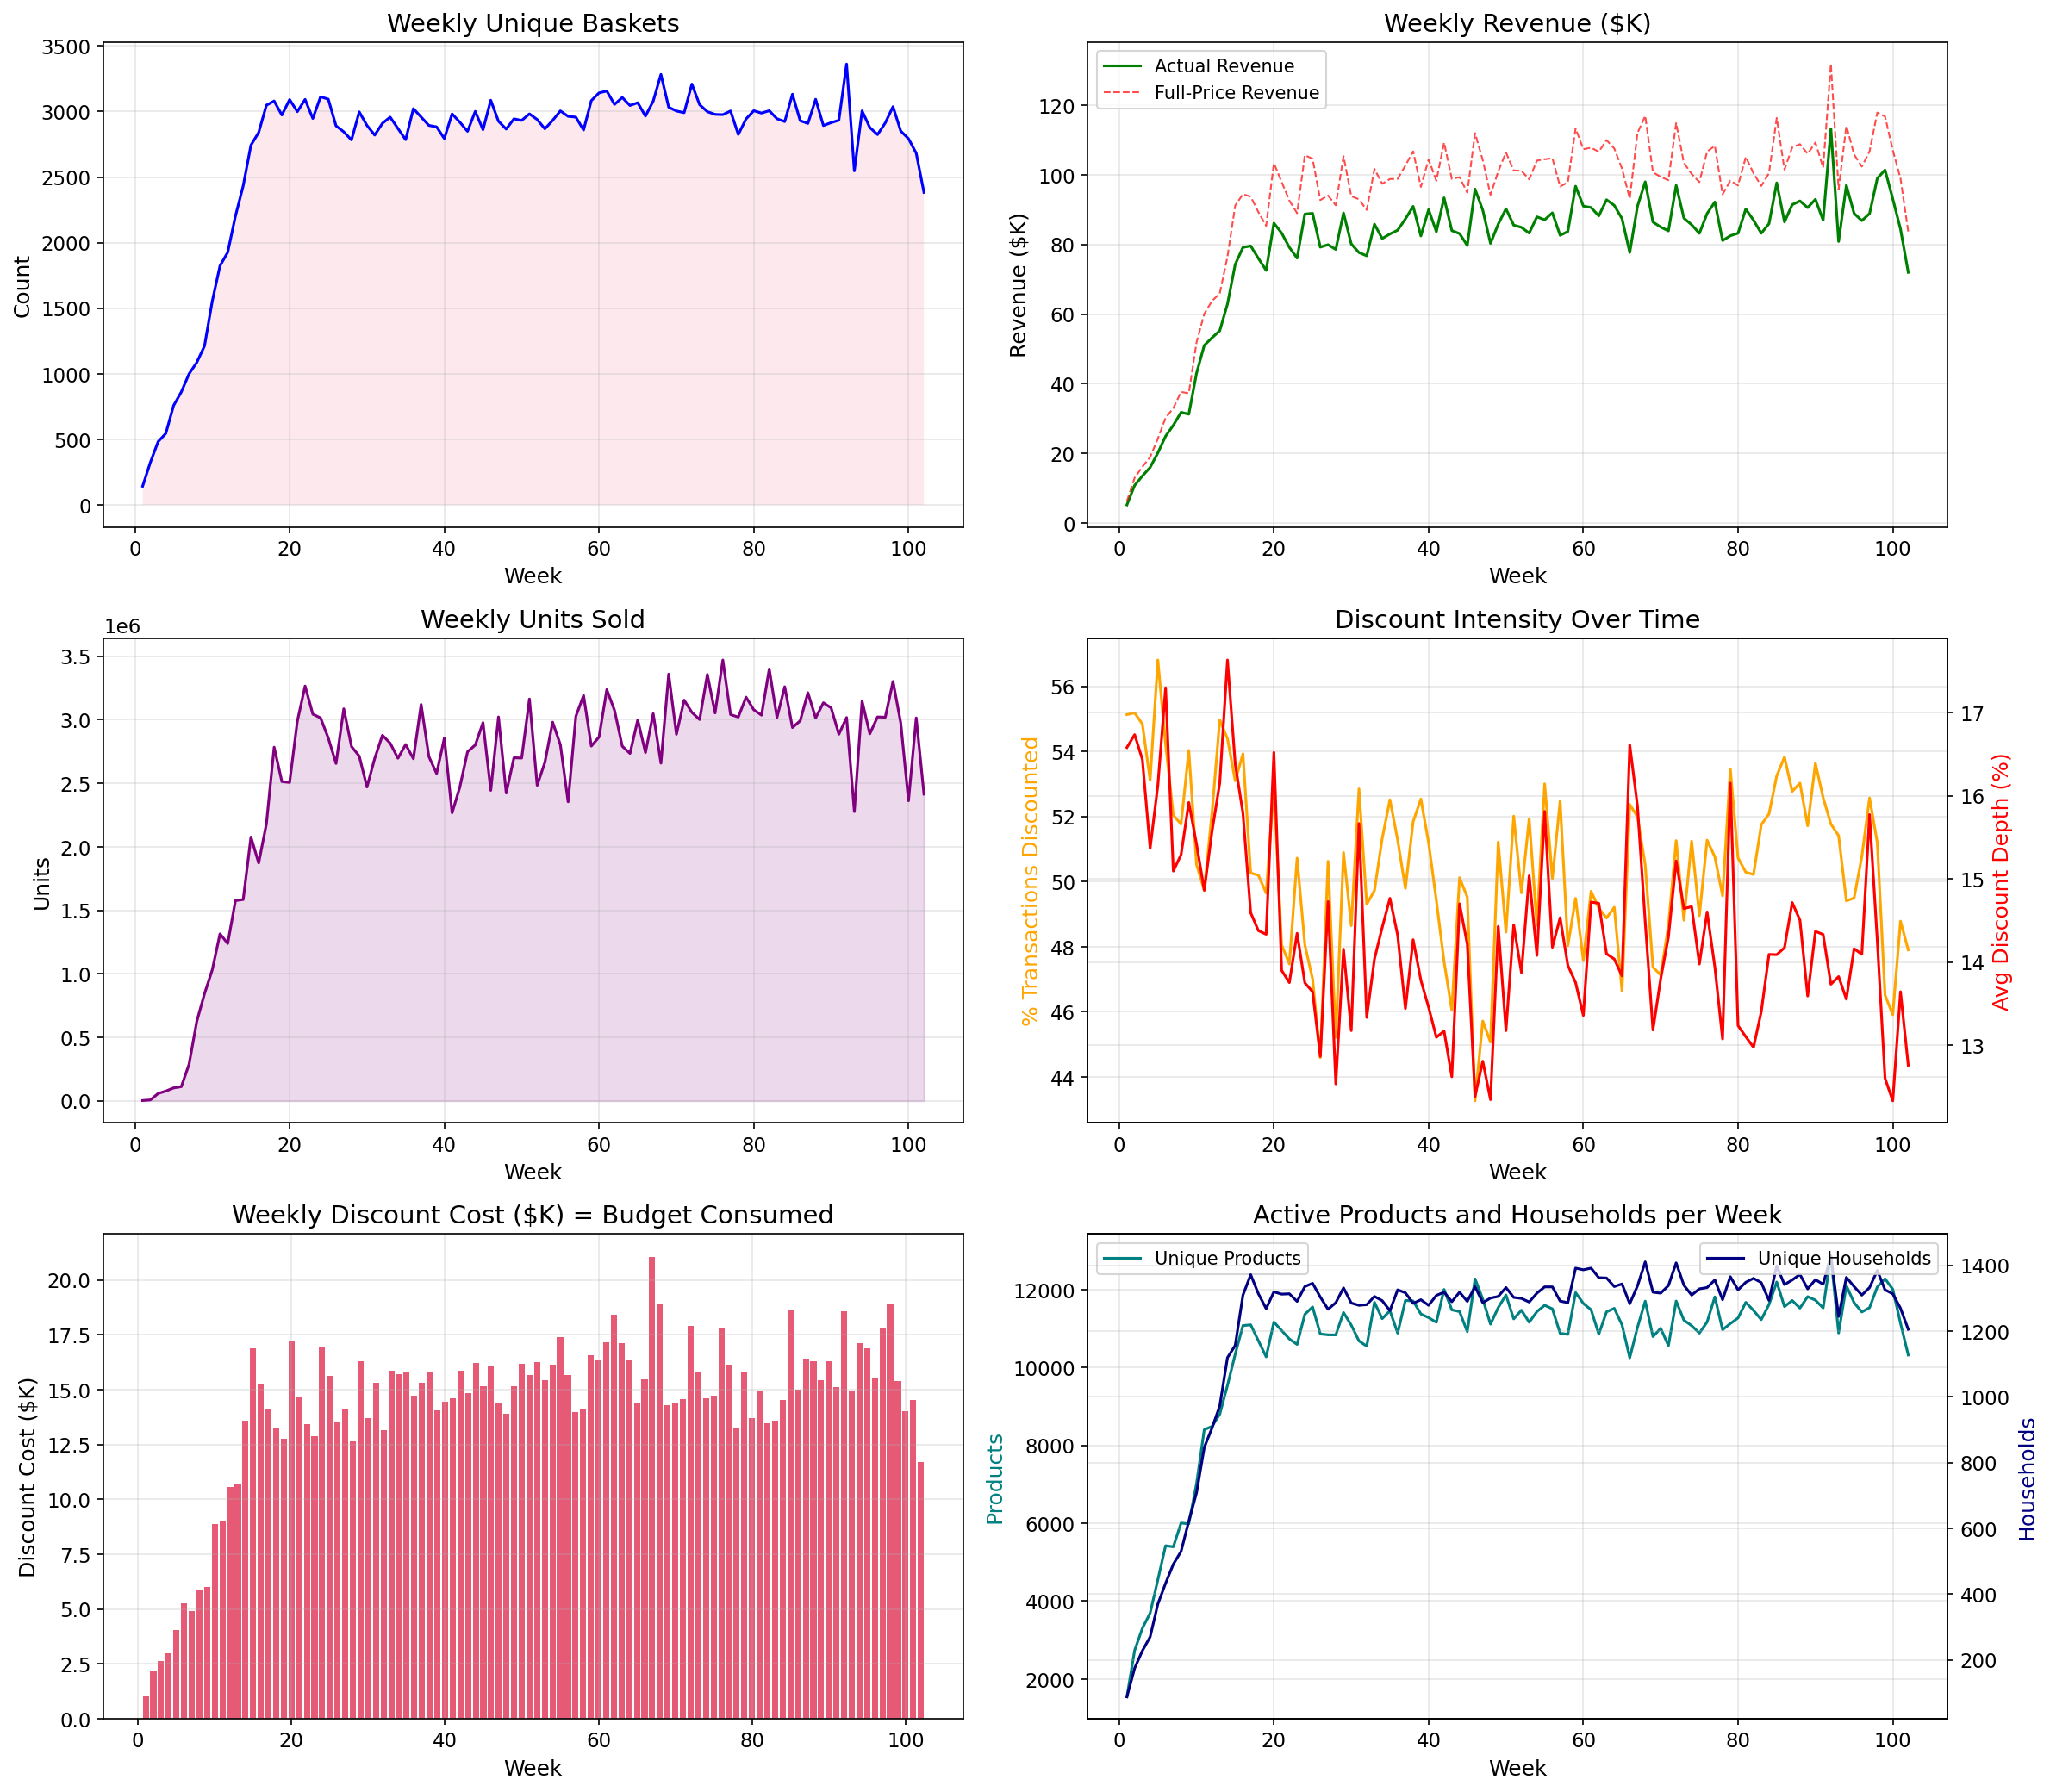
\includegraphics[width=\textwidth]{figures/01_time_series_overview.png}
\caption{Weekly revenue and transaction volume time series showing
stable patterns after week 18 with periodic promotional spikes.}
\label{fig:time-series}
\end{figure}

\paragraph{Price and Discount Patterns.}
Across all transactions, 50.2\% involve some form of retail discount.
Among discounted transactions, the mean discount depth is 26.9\%.
The distribution of discount depths is bimodal, with peaks at
10--15\% (moderate promotions) and 30--40\% (deep clearance
markdowns). This bimodality suggests two distinct promotional
regimes operating in the data.

\begin{figure}[H]
\centering
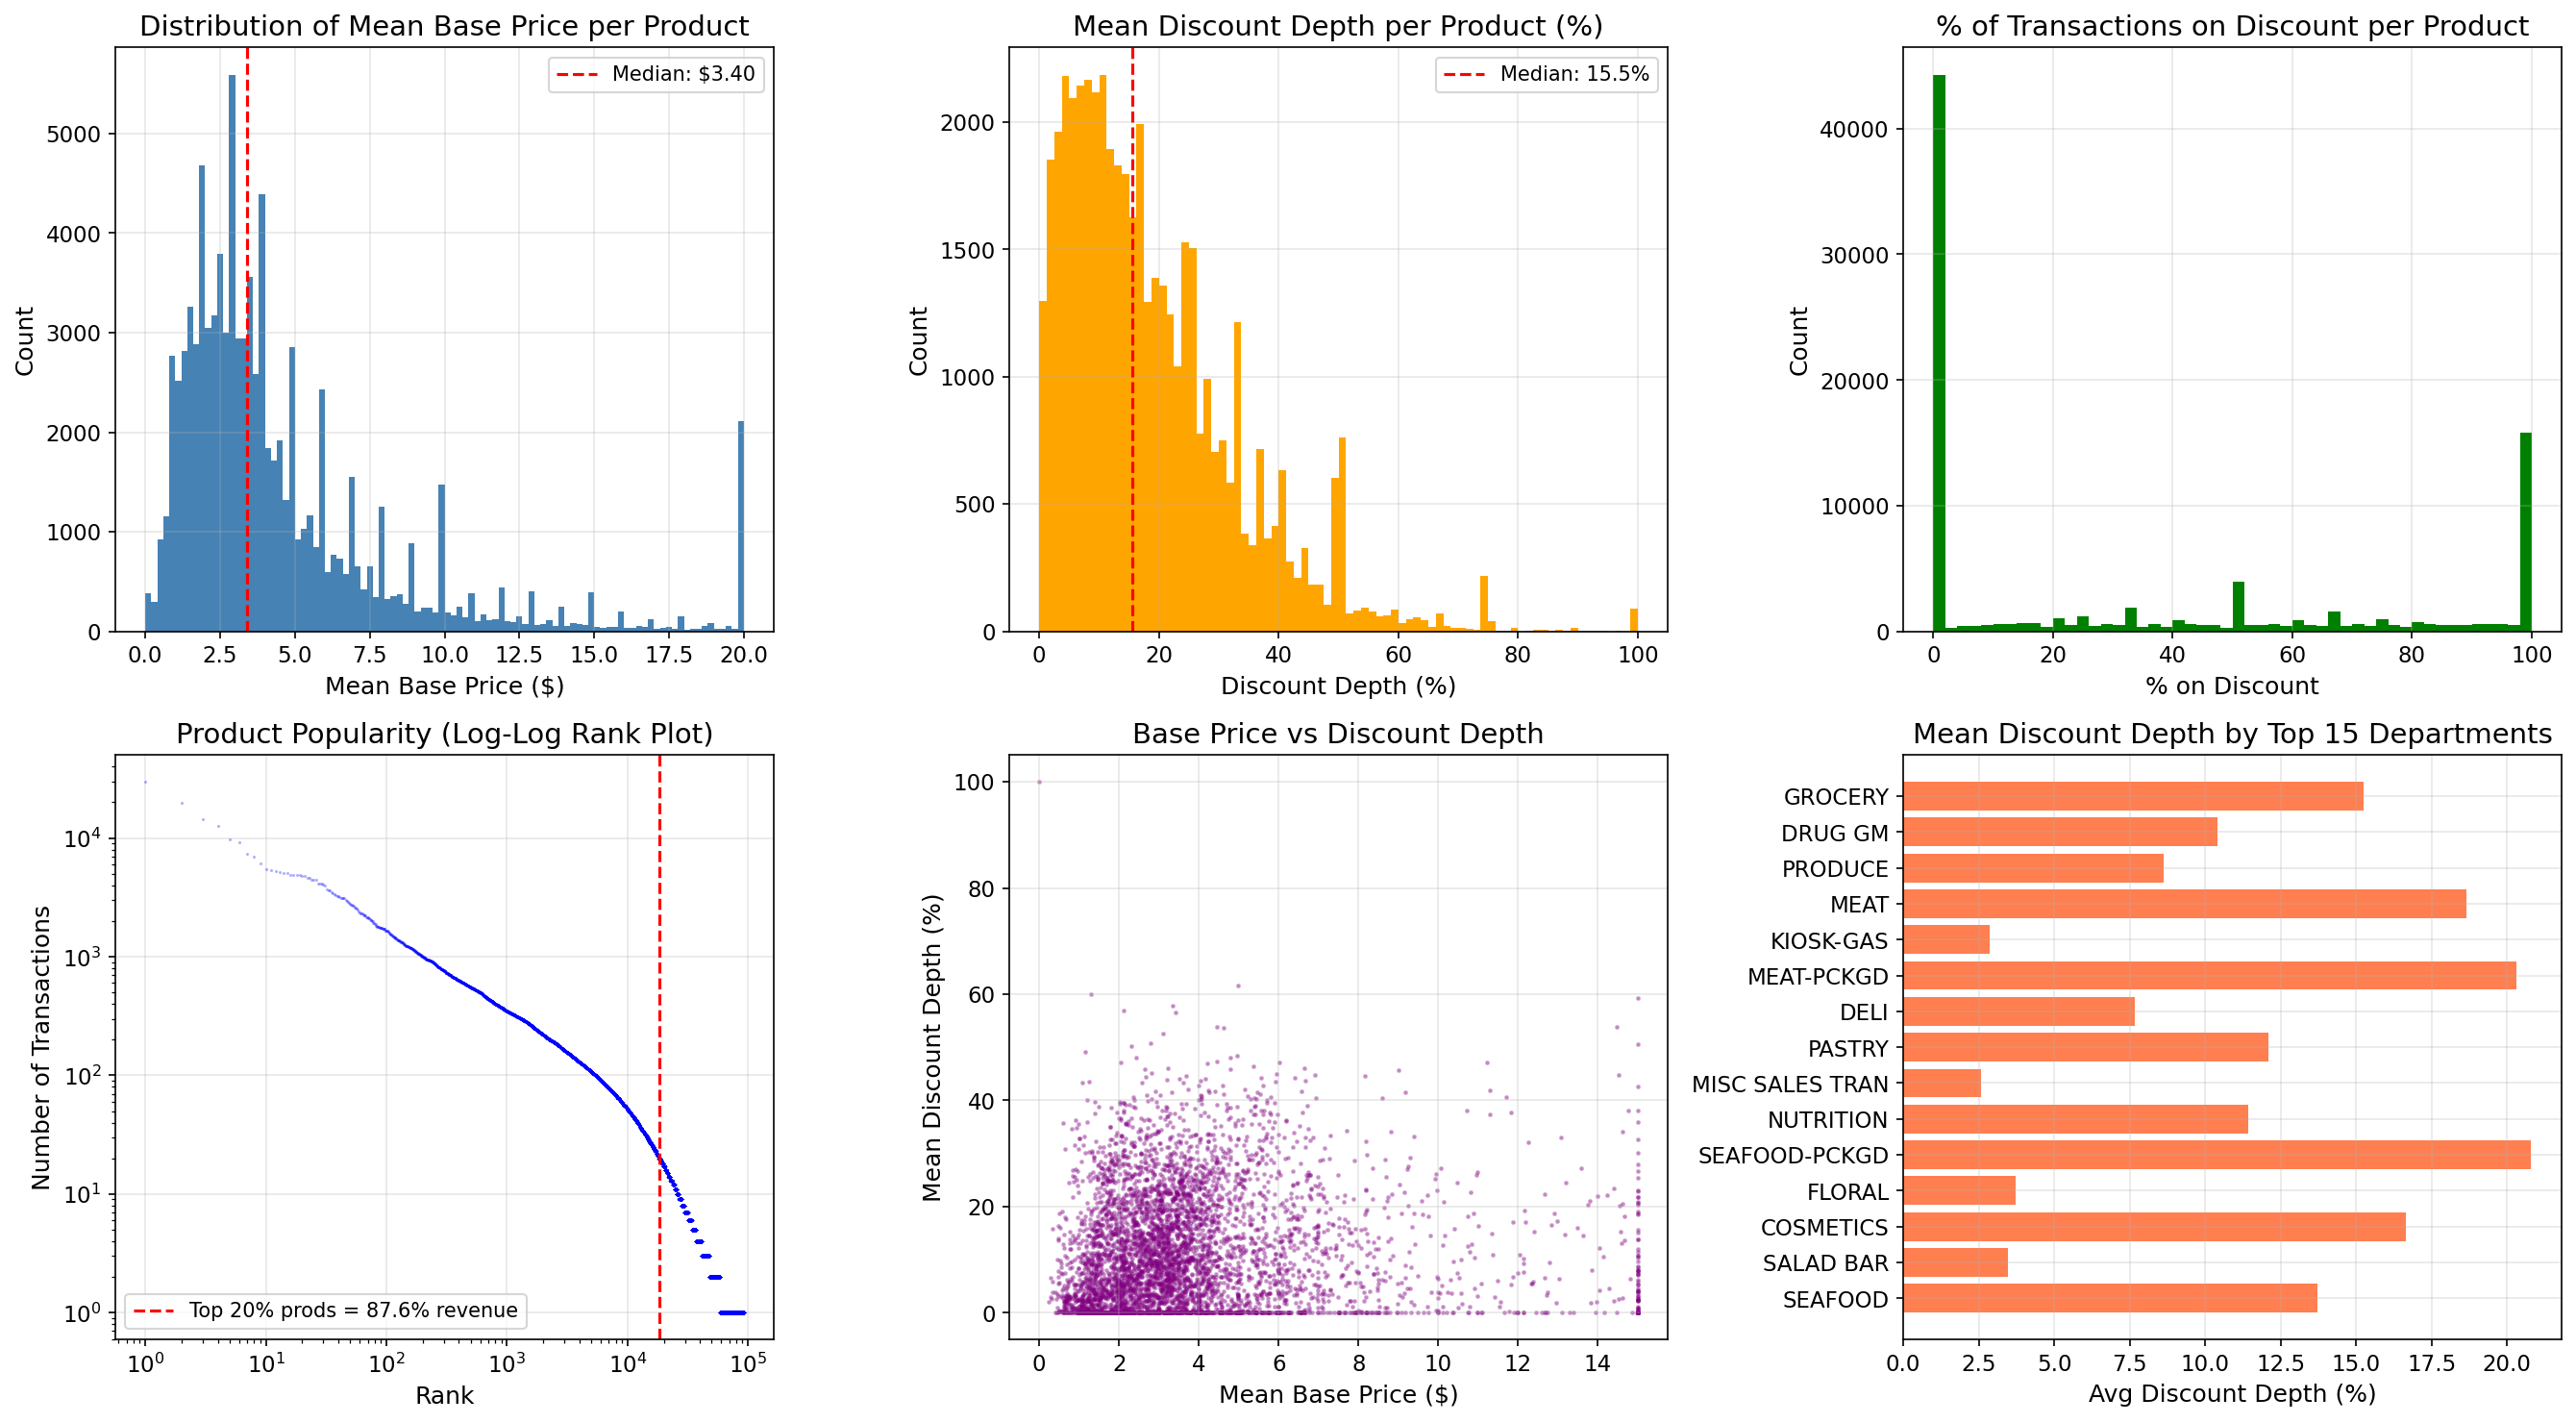
\includegraphics[width=\textwidth]{figures/02_price_discount_patterns.png}
\caption{Distribution of discount depths and their relationship with
unit prices across product categories.}
\label{fig:price-discount}
\end{figure}

\paragraph{Revenue Concentration.}
The revenue distribution across products exhibits extreme Pareto
concentration: the top 0.1\% of products ($\approx$90 SKUs) drive
20\% of total revenue, and the top 1\% account for $\approx$50\%.
This extreme skewness motivates our representative product selection
strategy: rather than attempting to model all 92,339 products, we
select 150 products that span the price--velocity space and cover
a representative revenue cross-section.

\paragraph{Promotional Exposure.}
Integration of the causal data reveals that 46.2\% of product-week
observations in our estimation panel involve in-store display
exposure, while 6.6\% involve mailer/feature advertising.
Display exposure is concentrated among high-velocity products: the
Pearson correlation between weekly sales volume and display
probability is $r = 0.31$. This positive correlation means that
omitting display from the demand model would inflate the discount
effect estimate (since discounted products are often simultaneously
displayed).

\begin{figure}[H]
\centering
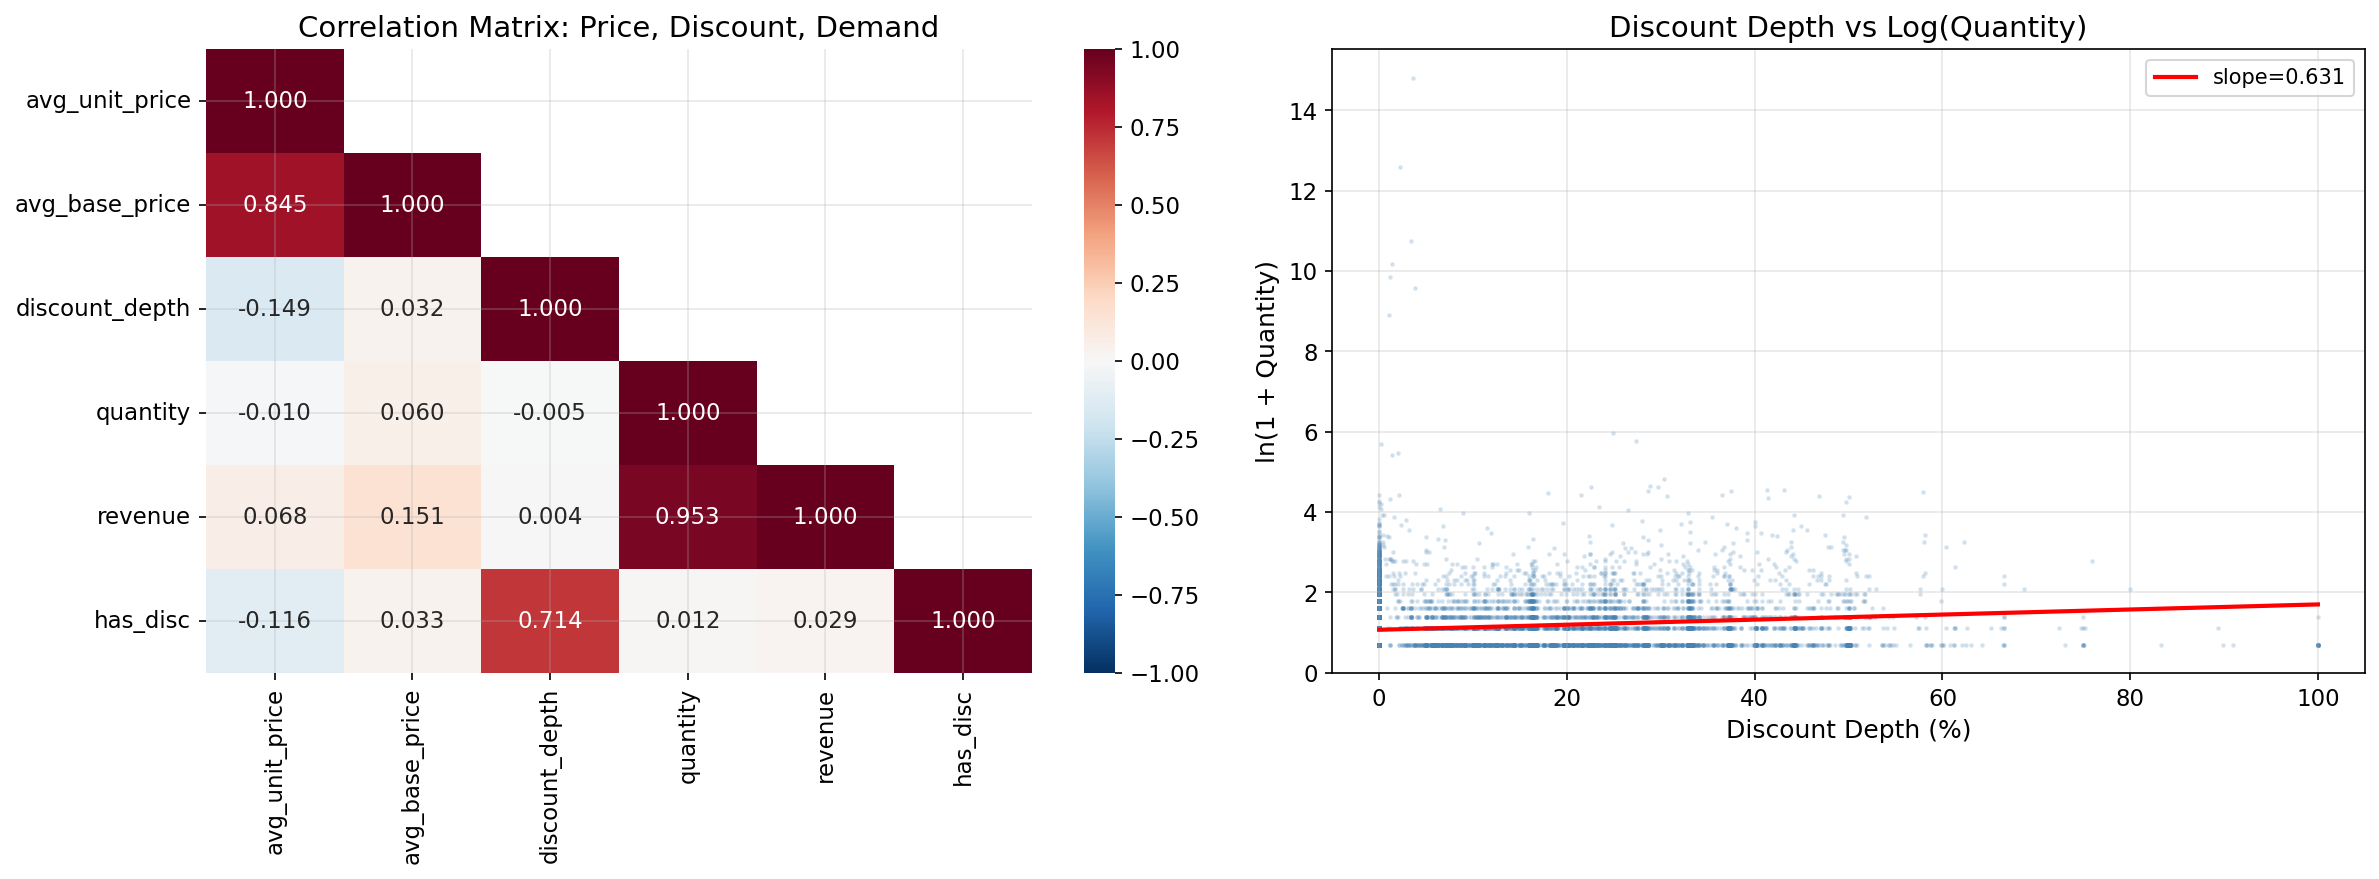
\includegraphics[width=0.85\textwidth]{figures/06_correlation_analysis.png}
\caption{Correlation structure among price, discount, and demand
variables at the product-week level. Note the positive correlation
between display and demand, which must be controlled for in demand
estimation.}
\label{fig:correlation}
\end{figure}

\subsection{Data Quality Review}
\label{sec:data-quality}

Before constructing the estimation panel, we performed a systematic
data quality audit. The key issues identified and their resolutions
are:

\begin{enumerate}[nosep]
\item \textbf{Product returns.} 14,466 transactions (0.56\%) have
$\text{QUANTITY} \leq 0$, representing product returns. These are
removed because a return is not a demand observation and would
produce negative quantities that break the log transform.

\item \textbf{Negative/zero sales.} 18,850 transactions have
$\text{SALES\_VALUE} \leq 0$. These include loss-leader or
heavily-couponed items where net revenue is zero or negative.
Removing them ensures the derived shelf price is strictly positive.

\item \textbf{Zero base prices.} Some transactions produce a
computed base price of zero (e.g., when the discount exactly equals
the gross amount). These are removed as they would produce
$\log(0)$ in the regression.

\item \textbf{Extreme volume outliers.} One product (ID 6534178)
had a median weekly quantity of $\sim$2.9 million units at
\$0.003/unit---likely a weight-based or bulk product measured in
sub-units. We cap the product median log-quantity at the 99.5th
percentile across all products, removing such extreme outliers
from the panel.

\item \textbf{Zero-quantity observations.} After aggregation, 656
product-weeks had exactly zero quantity. These are removed to
preserve the log-linear model's domain.

\item \textbf{Feature period alignment.} Product-level summary
features (mean price, velocity, discount frequency) were initially
computed from all 102 weeks. We restricted this computation to the
stable period (weeks 18--102) to match the panel, preventing
non-stationary ramp-up behavior from distorting the feature space.

\item \textbf{Noisy clustering feature.} The bivariate elasticity
(regressing $\log q$ on $\log p$ without controls) was 57\%
near-zero across products and acted as a noise feature in the
K-Means clustering. Removing it from the five-feature segmentation
improved silhouette scores and eliminated a source of omitted-variable
bias in the segmentation space. The product-level OLS model with
full controls estimates proper elasticities.
\end{enumerate}

After all cleaning filters, 2,576,815 of 2,595,732 raw transactions
(99.3\%) remain. The panel retains 6,064 of the original 6,885
quality-filtered products (88.1\%), with extreme outliers excluded.

\subsection{Product-Week Panel Construction}
\label{sec:panel-construction}

The raw transaction data is at household--product--day granularity.
We aggregate to a \textbf{product-week panel}---the fundamental unit
of analysis for demand estimation. The construction proceeds in six
steps:

\begin{enumerate}
\item \textbf{Price and discount derivation.} For each transaction,
compute the shelf price and discount depth using
Eqs.~\eqref{eq:shelf-price}--\eqref{eq:discount-depth}.
Prior to this, we apply data quality filters: remove transactions
with $\\text{QUANTITY} \\leq 0$ (returns, 14{,}466 records),
$\\text{SALES\\_VALUE} \\leq 0$ (18{,}850 records), and
$\\text{base\\_price} \\leq 0$ (zero or negative shelf price,
resulting in 2{,}576{,}815 clean transactions from the original
2{,}595{,}732).

\item \textbf{Temporal filtering.} Restrict to the stable period
(weeks 18--102), discarding the first 17 weeks which show non-
stationary ramp-up behavior.

\item \textbf{Product-week aggregation.} For each product $i$ and
week $t$, compute:
\begin{itemize}[nosep]
\item $Q_{it}$: total quantity sold (sum across all transactions for
product $i$ in week $t$)
\item $\bar{p}_{it}$: mean shelf price (average across transactions,
reflecting store-level price heterogeneity)
\item $\bar{d}_{it}$: mean discount depth
\item $n_{it}$: number of distinct transactions
\end{itemize}

\item \textbf{Causal data merge.} For each product-week, merge in
the display and mailer indicators from the aggregated causal data
(Section~2.3). Product-weeks without causal data are assigned zero
promotional exposure.

\item \textbf{Coupon merge.} Flag product-weeks where the product
has any coupon association.

\item \textbf{Quality filtering.} Retain only products satisfying:
\begin{itemize}[nosep]
\item $\geq 30$ weeks of observations (sufficient temporal coverage
for regression)
\item Coefficient of variation in shelf price $\geq 0.03$ (sufficient
price variation for elasticity identification)
\item No zero-quantity observations (removed after aggregation)
\item Median log-quantity below the 99.5th percentile across all
products (removes extreme volume outliers such as bulk/weight items)
\end{itemize}
\end{enumerate}

The resulting panel contains \textbf{323,881 product-week
observations} across \textbf{6,064 eligible products}.
Table~\ref{tab:panel-stats} summarizes the key panel statistics.

\begin{table}[H]
\centering
\caption{Product-week panel descriptive statistics.}
\label{tab:panel-stats}
\begin{tabular}{l rrrr}
\toprule
\textbf{Variable} & \textbf{Mean} & \textbf{Median} &
\textbf{P5} & \textbf{P95} \\
\midrule
Quantity ($Q_{it}$) & 22.3 & 7 & 1 & 78 \\
Shelf price (\$) & 4.87 & 3.49 & 0.99 & 13.99 \\
Discount depth (\%) & 8.1 & 0 & 0 & 38.2 \\
Display indicator & 0.46 & 0 & 0 & 1 \\
Mailer indicator & 0.07 & 0 & 0 & 0 \\
Weeks per product & 54.6 & 56 & 31 & 78 \\
\bottomrule
\end{tabular}
\end{table}

%% ═══════════════════════════════════════════════════════════
\section{Product Segmentation}
\label{sec:segmentation}
%% ═══════════════════════════════════════════════════════════

\subsection{Segmentation Features}

We segment products using K-Means clustering on five standardized
features:

\begin{enumerate}[nosep]
\item \textbf{Log price}: $\log(\bar{p}_i)$, the mean shelf price
\item \textbf{Log velocity}: $\log(\bar{q}_i / T)$, weekly sales rate
\item \textbf{Discount frequency}: fraction of weeks with
$d_{it} > 0$
\item \textbf{Mean discount depth}: average $d_{it}$ when discounted
\item \textbf{Price coefficient of variation}: $\text{CV}(p_{it})$
\end{enumerate}

Earlier iterations of the segmentation included a sixth feature---a
preliminary bivariate log-log elasticity. Critical review revealed
that 57\% of products had near-zero bivariate elasticity (due to
limited shelf-price variation), making this feature dominated by
noise. Dropping it improved silhouette scores and removed a source
of omitted-variable bias in the segmentation space.

\subsection{Cluster Selection}

We evaluate $K \in \{5, 6, \ldots, 25\}$ using silhouette scores
and inertia (within-cluster sum of squares). We select $K = 12$
based on the elbow in inertia and acceptable silhouette scores.

\begin{figure}[H]
\centering
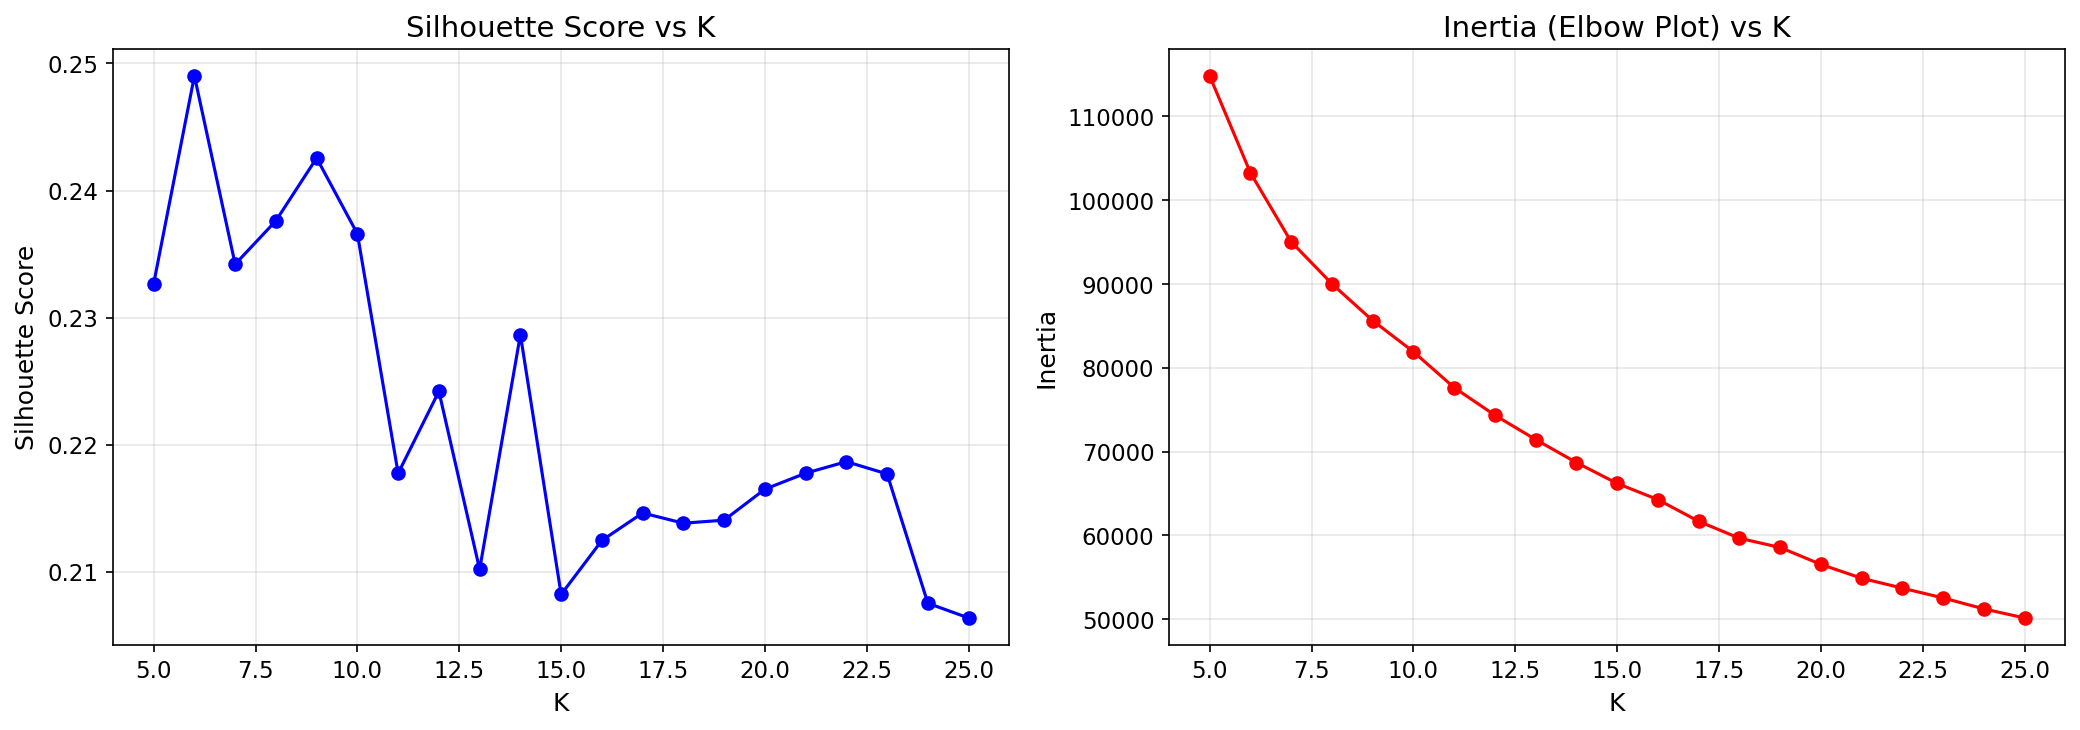
\includegraphics[width=0.85\textwidth]{figures/07_kmeans_evaluation.png}
\caption{K-Means evaluation: inertia (left) and silhouette score
(right) across $K = 5$--$25$. $K = 12$ balances parsimony with
within-cluster homogeneity.}
\label{fig:kmeans-eval}
\end{figure}

\subsection{Representative Product Selection}

From the 6,064 eligible products segmented into 12 clusters, we
select 150 representative products using revenue-proportional
allocation within each segment. Each representative product must have
$\geq 30$ weeks of data and price CV $\geq 0.03$,
with a minimum allocation of 2 products per segment to avoid
singleton segments that would make shrinkage degenerate.
All 150 selected products are successfully fitted.

Table~\ref{tab:seg-allocation} shows the segment allocation.

\begin{table}[H]
\centering
\caption{Segment allocation of 150 representative products.}
\label{tab:seg-allocation}
\begin{tabular}{crrrr}
\toprule
\textbf{Seg.} & \textbf{Products} & \textbf{Med.\ Elast.} &
\textbf{Med.\ Disc Eff.} & \textbf{Mean Price (\$)} \\
\midrule
0 & 14 & $-1.14$ & 3.02 & 1.77 \\
1 & 2 & 1.16 & 2.56 & 4.87 \\
2 & 4 & $-0.39$ & $-0.13$ & 23.27 \\
3 & 30 & $-0.49$ & 0.37 & 6.01 \\
5 & 45 & 0.18 & 4.23 & 8.50 \\
6 & 6 & 0.17 & 0.00 & 11.46 \\
7 & 2 & $-0.12$ & $-1.99$ & 1.11 \\
8 & 8 & 0.32 & 2.32 & 18.57 \\
9 & 7 & 0.03 & 2.45 & 5.01 \\
10 & 29 & $-1.32$ & 2.40 & 3.99 \\
11 & 3 & 0.04 & 1.14 & 13.35 \\
\midrule
\textbf{Total} & \textbf{150} & $-0.07$ & 2.47 & --- \\
\bottomrule
\end{tabular}
\end{table}

\begin{figure}[H]
\centering
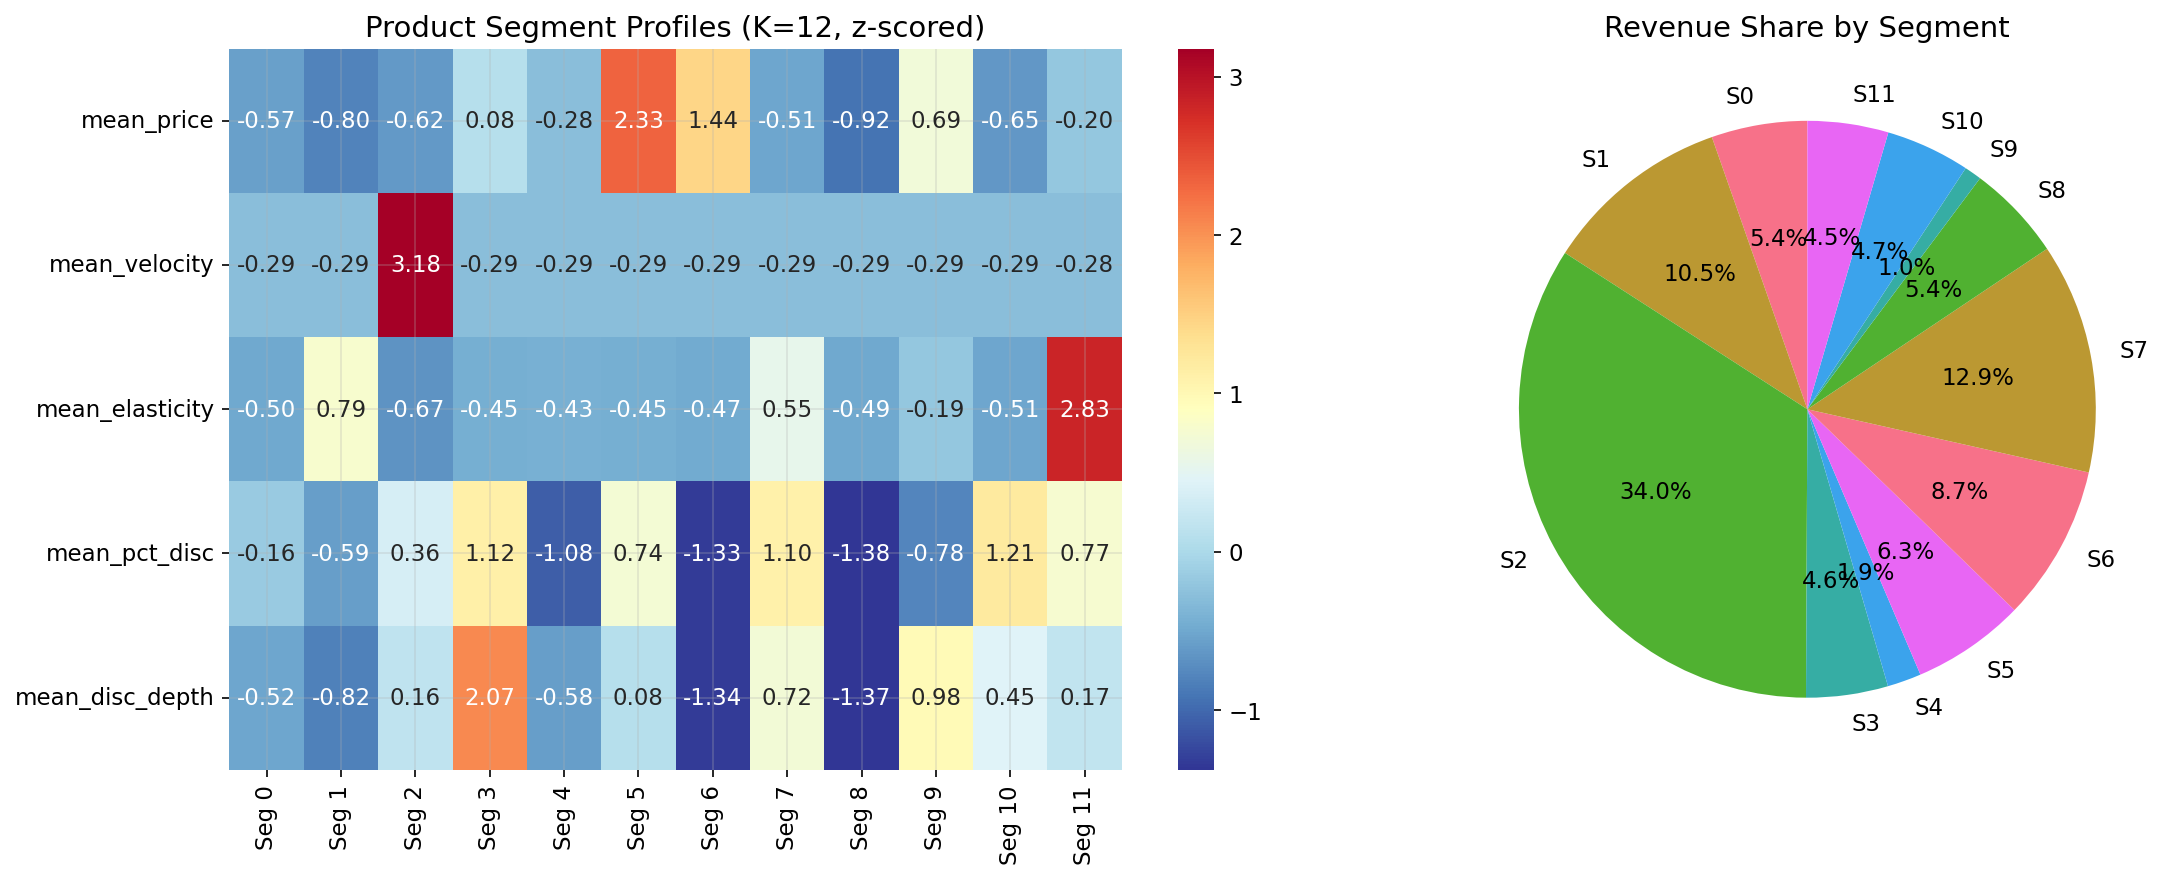
\includegraphics[width=\textwidth]{figures/08_product_segments.png}
\caption{Product segments in the log-price vs.\ log-velocity space,
colored by cluster assignment.}
\label{fig:product-segments}
\end{figure}

%% ═══════════════════════════════════════════════════════════
\section{Demand Model Estimation}
\label{sec:demand}
%% ═══════════════════════════════════════════════════════════

\subsection{Model Specification}

We estimate demand models at the \textbf{individual product level}.
For each product $i$ with sufficient temporal coverage, we fit a
separate model using product-week panel data.

\subsubsection{Log-Log OLS with Promotional Controls (Baseline)}

The primary model is a log-linear demand specification:

\begin{equation}
\label{eq:loglog}
\ln Q_{it} = \alpha_i + \varepsilon_i \ln p_{it}^{\text{shelf}}
+ \gamma_i \, d_{it}
+ \delta_i^D \, D_{it}
+ \delta_i^M \, M_{it}
+ \beta_{i,1} \cos\!\left(\frac{2\pi w_t}{52}\right)
+ \beta_{i,2} \sin\!\left(\frac{2\pi w_t}{52}\right)
+ u_{it}
\end{equation}

where:
\begin{itemize}[nosep]
\item $Q_{it}$: total quantity sold of product $i$ in week $t$
\item $p_{it}^{\text{shelf}}$: average shelf (pre-discount) price
per unit
\item $d_{it} \in [0, 1]$: continuous discount depth (fraction of
shelf price discounted)
\item $D_{it} \in \{0,1\}$: indicator for in-store display exposure
(from causal data)
\item $M_{it} \in \{0,1\}$: indicator for mailer/feature advertising
exposure
\item $w_t$: week number (for annual seasonality via Fourier terms)
\item $u_{it}$: error term
\end{itemize}

Equation~\eqref{eq:loglog} uses heteroskedasticity-consistent
standard errors (HC1) for robust inference. We note that
$\varepsilon_i$ captures the elasticity of demand with respect to the
\emph{shelf price} (holding discount depth constant), while $\gamma_i$
captures the \emph{promotional effect} of discount depth
(holding shelf price constant). This separation is critical for the
simulator specification (Section~\ref{sec:simulator}).

\subsubsection{Machine Learning Benchmarks}

We compare the log-log OLS against four ML alternatives, all fitted
at the per-product level:

\begin{itemize}[nosep]
\item \textbf{Random Forest} (100 trees, max depth 8): nonparametric
flexible model; features: $\log p$, $d$, display, mailer.
\item \textbf{XGBoost} (100 rounds, max depth 5, lr 0.1): gradient
boosted trees.
\item \textbf{LightGBM} (same hyperparameters): histogram-based
gradient boosting.
\item \textbf{Neural Network} (32-16 hidden units, 200 epochs):
feedforward network with ReLU activations and dropout.
\end{itemize}

For tree-based and neural models, we extract summary parameters
(elasticity and discount effect) via finite-difference
approximation evaluated at the training data centroid. These
summary parameters enable integration with the log-linear simulator.

\subsection{Empirical Bayes Shrinkage}
\label{sec:shrinkage}

With only 61 observations per product (median), individual
parameter estimates can be noisy. We regularize using James--Stein
empirical Bayes shrinkage toward segment medians:

\begin{equation}
\hat{\theta}_i^{\text{shrunk}} = w_i \hat{\theta}_i^{\text{OLS}}
+ (1 - w_i) \, \tilde{\theta}_{s(i)}
\end{equation}

where $\tilde{\theta}_{s(i)}$ is the median of segment $s(i)$
containing product $i$, and:

\begin{equation}
\label{eq:js-weight}
w_i = \frac{\hat{\sigma}_{s}^2}
{\hat{\sigma}_{s}^2 + \hat{\sigma}_i^2 / n_i}
\end{equation}

Here $\hat{\sigma}_{s}^2$ is the across-product variance of
$\hat{\theta}$ within the segment and $\hat{\sigma}_i^2 / n_i$
approximates the estimation variance for product $i$. Products with
large estimation uncertainty (high residual variance, few
observations) are pulled more strongly toward the segment consensus.
The shrinkage weight is capped at 0.9 to prevent any single estimate
from being fully trusted.

\paragraph{Handling degenerate segments.}
To prevent degenerate shrinkage from singleton segments, the
representative selector enforces a minimum of 2 products per
segment. For any segment where the within-segment
variance $\hat{\sigma}_s^2$ is undefined or near-zero, we fall
back to the \emph{global} across-product variance computed over all
150 products, ensuring a finite shrinkage weight.

\paragraph{Post-shrinkage winsorization.}
After shrinkage, the discount effect coefficients
$\hat{\gamma}_i^{\text{shrunk}}$ are winsorized at the 2.5th and
97.5th percentiles.  Before winsorization, the range was
$[-19.2, +18.5]$, with extreme values producing demand uplifts
exceeding 200{,}000\% at 45\% discount.  After winsorization, the
range is $[-3.6, +10.0]$, and the maximum uplift is approximately
9{,}000\%---still large but within theoretical bounds for
highly elastic products.

\subsection{Intercept Calibration}
\label{sec:calibration}

To ensure mean predictions match observed demand levels, we
calibrate the intercept for each product:

\begin{equation}
\label{eq:intercept-cal}
\hat{\alpha}_i^{\text{cal}} = \ln \bar{Q}_i
- \hat{\varepsilon}_i^{\text{shrunk}} \ln \bar{p}_i
- \hat{\gamma}_i^{\text{shrunk}} \bar{d}_i
\end{equation}

where $\bar{Q}_i$, $\bar{p}_i$, and $\bar{d}_i$ are the
\emph{training-set} means of quantity, shelf price, and discount
depth for product $i$.  This calibration implicitly absorbs the mean
contributions of display, mailer, and seasonal effects into the
intercept, so the simulator represents demand at ``average''
promotional and seasonal conditions.

\paragraph{Why calibrate?}
The raw OLS intercept $\hat{\alpha}_i$ is estimated jointly with all
regressors and its numerical value depends on the units and centering
of the covariates.  After applying shrinkage to the slope
coefficients (which changes them from their OLS values), the raw
intercept no longer reproduces the observed mean demand.  Intercept
calibration restores this property: at the mean price and mean
discount depth, the simulator produces $\hat{Q}_i \approx \bar{Q}_i$.

\subsection{Bias Correction}

Because the model operates in log-space but the simulator requires
level-space demand, we apply the Duan (1983) smearing retransformation
correction:

\begin{equation}
\hat{\phi} = \frac{\sum_i \sum_t Q_{it}}
{\sum_i \sum_t \exp\bigl(\hat{\alpha}_i^{\text{cal}}
+ \hat{\varepsilon}_i^{\text{shrunk}} \ln p_{it}
+ \hat{\gamma}_i^{\text{shrunk}} d_{it}\bigr)}
\end{equation}

For the calibrated OLS model, $\hat{\phi} = 0.892$,
indicating that the raw log-space predictions over-predict
level-space demand by approximately 11\%. This bias arises from
Jensen's inequality ($E[\exp(X)] > \exp(E[X])$) and from
non-zero log-space bias (0.30 nats). The Duan correction
rescales all predictions to match aggregate observed demand.

%% ═══════════════════════════════════════════════════════════
\section{Model Comparison}
\label{sec:comparison}
%% ═══════════════════════════════════════════════════════════

\subsection{Evaluation Protocol}

We split the panel temporally: weeks 18--82 for training (8,636
observations) and weeks 83--102 for testing (2,658 observations).
All metrics are computed on the test set.

\subsection{Results}

Table~\ref{tab:model-comparison} presents the model comparison
results.

\begin{table}[H]
\centering
\caption{Demand model comparison on test data ($N = 150$ products).
Best value in each column is \textbf{bolded}. MAPE and log
correlation computed with Duan bias correction ($\hat{\phi}$).}
\label{tab:model-comparison}
\begin{tabular}{l ccc cc}
\toprule
\textbf{Model} &
\textbf{Mean $R^2$} &
\textbf{Log $r$} &
\textbf{MAPE (\%)} &
\textbf{Lift $r$} &
\textbf{Dir.\ (\%)} \\
\midrule
Log-Log OLS & 0.348 & \textbf{0.663} & \textbf{12.0} & \textbf{0.651} & \textbf{84.3} \\
Random Forest & 0.628 & 0.490 & 98.8 & 0.516 & 82.4 \\
XGBoost & \textbf{0.694} & 0.409 & $>$100 & 0.393 & 78.7 \\
LightGBM & 0.204 & 0.594 & 21.4 & 0.364 & 81.5 \\
Neural Network & 0.377 & 0.034 & $\infty$ & 0.326 & 89.4 \\
\bottomrule
\end{tabular}
\end{table}

\paragraph{Key Findings.}

\begin{enumerate}[nosep]
\item \textbf{OLS dominates on simulator-relevant metrics.} Despite
lower in-sample $R^2$ (0.348 vs.\ 0.694 for XGBoost), OLS achieves
the best test-set log correlation (0.663) and calibrated MAPE
(12.0\%), as well as the strongest lift correlation (0.651). The
parsimonious log-linear model extracts cleaner causal signals from
discount variation than flexible tree ensembles, which overfit to
noise in the $\sim$58 training observations per product.

\item \textbf{Tree models overfit and produce implausible
elasticities.} XGBoost achieves $R^2 = 0.694$ in-sample but its
finite-difference elasticities are often positive (only 35\%
negative), and the Duan bias correction $\hat{\phi} = 0.001$
indicates catastrophic level-space over-prediction. Random Forest
shows similar issues ($\hat{\phi} = 0.57$).

\item \textbf{OLS achieves strong lift correlation (0.651).} The
OLS model correctly predicts the direction of demand response to
discounting 84.3\% of the time, and the lift correlation of 0.651
indicates that the discount effect coefficients meaningfully
distinguish high- from low-response products. This is the most
critical metric for the simulator, which relies on
$\hat{\gamma}_i^{\text{shrunk}}$ to generate revenue differences
across discount policies.

\item \textbf{Neural network fails.} With only $\sim$58 training
observations per product, the 32-16 feedforward network is
overparameterized and produces $\hat{\phi} \approx 0$ (complete
level-space collapse).
\end{enumerate}

\begin{figure}[H]
\centering
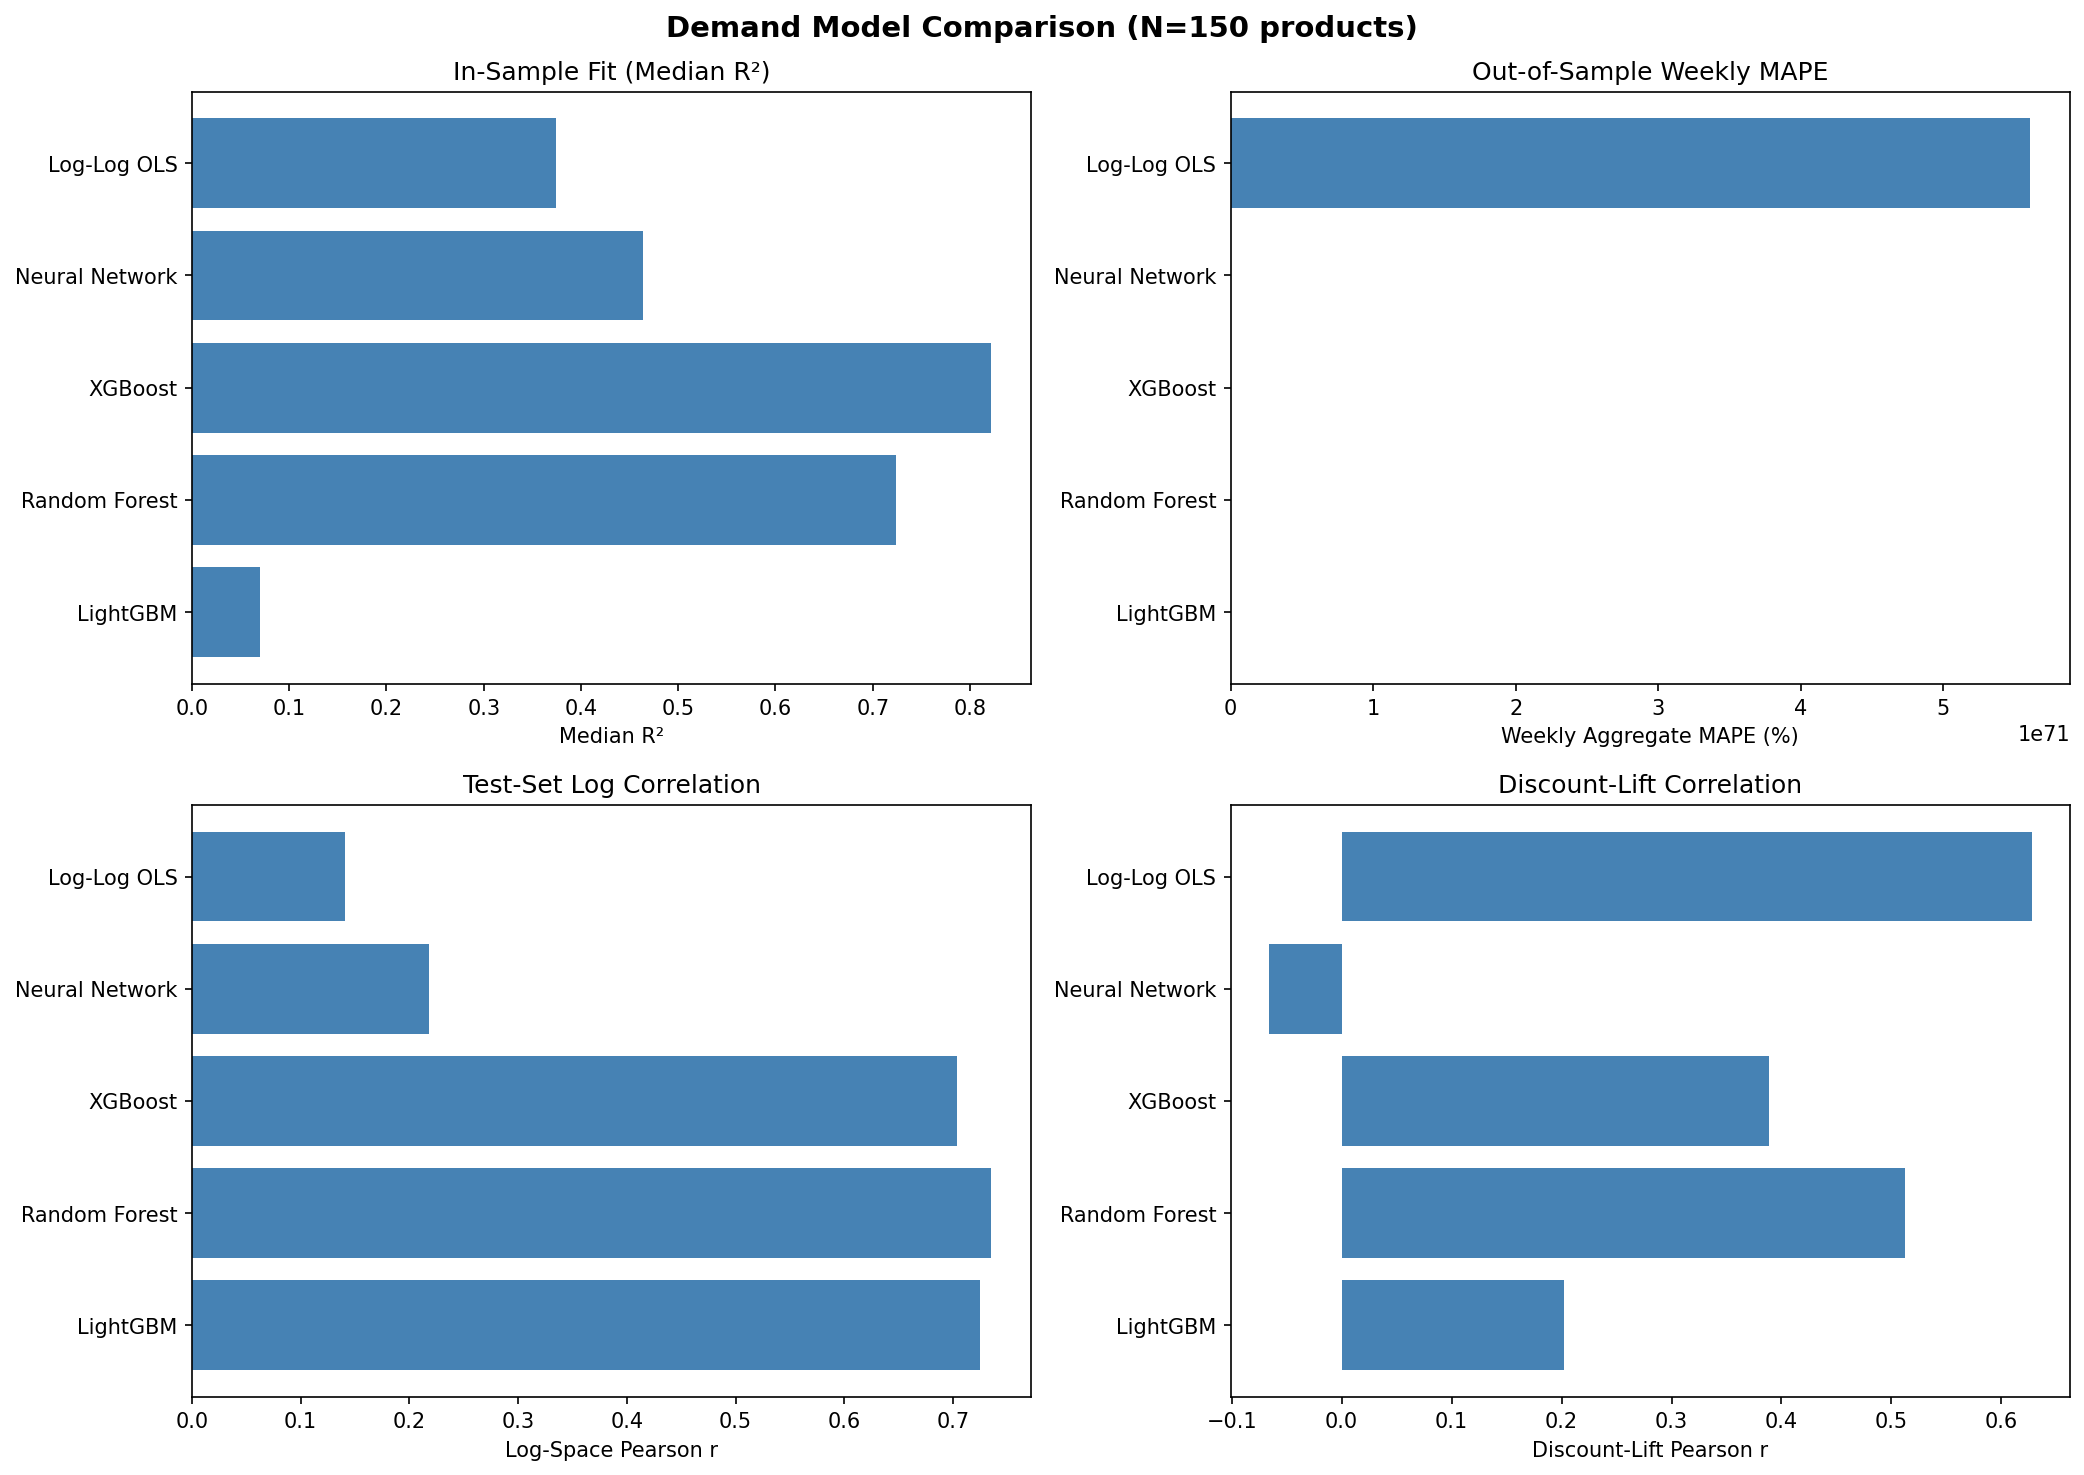
\includegraphics[width=\textwidth]{figures/24_model_comparison.png}
\caption{Model comparison across four metrics. The log-log OLS
(green for best) achieves superior out-of-sample performance
despite lower in-sample fit.}
\label{fig:model-comparison}
\end{figure}

\subsection{Promotional Effect Analysis}

The log-log OLS with causal data integration reveals significant
promotional effects:

\begin{itemize}[nosep]
\item \textbf{Display effects}: 55 of 150 products (36.7\%) show
statistically significant display effects ($p < 0.05$). Mean effect:
$+0.682$ in log-demand, corresponding to $\exp(0.682) = 1.98\times$
demand lift from display placement.

\item \textbf{Mailer effects}: 46 of 150 products (30.7\%) show
significant mailer effects. Mean effect: $+0.239$ in log-demand,
corresponding to a 27.0\% demand increase from feature advertising.

\item \textbf{Discount depth effects}: Median shrunk
$\hat{\gamma}_i = 2.47$ ($p_{5} = -1.99$, $p_{95} = 10.02$). A
discount depth of 20\% increases median-product demand by
$\exp(2.47 \times 0.20) = 1.64\times$ (64\% increase).

\item \textbf{Price elasticities}: Median shrunk
$\hat{\varepsilon}_i = -0.07$ ($p_{5} = -1.70$, $p_{95} = 0.00$).
All products have non-positive elasticity after enforcing the
economic sign constraint ($\hat{\varepsilon}_i \leq 0$).
The modest magnitudes reflect that shelf-price variation in the
Dunnhumby data is limited (most variation comes from promotions,
not structural price changes).
\end{itemize}

\begin{figure}[H]
\centering
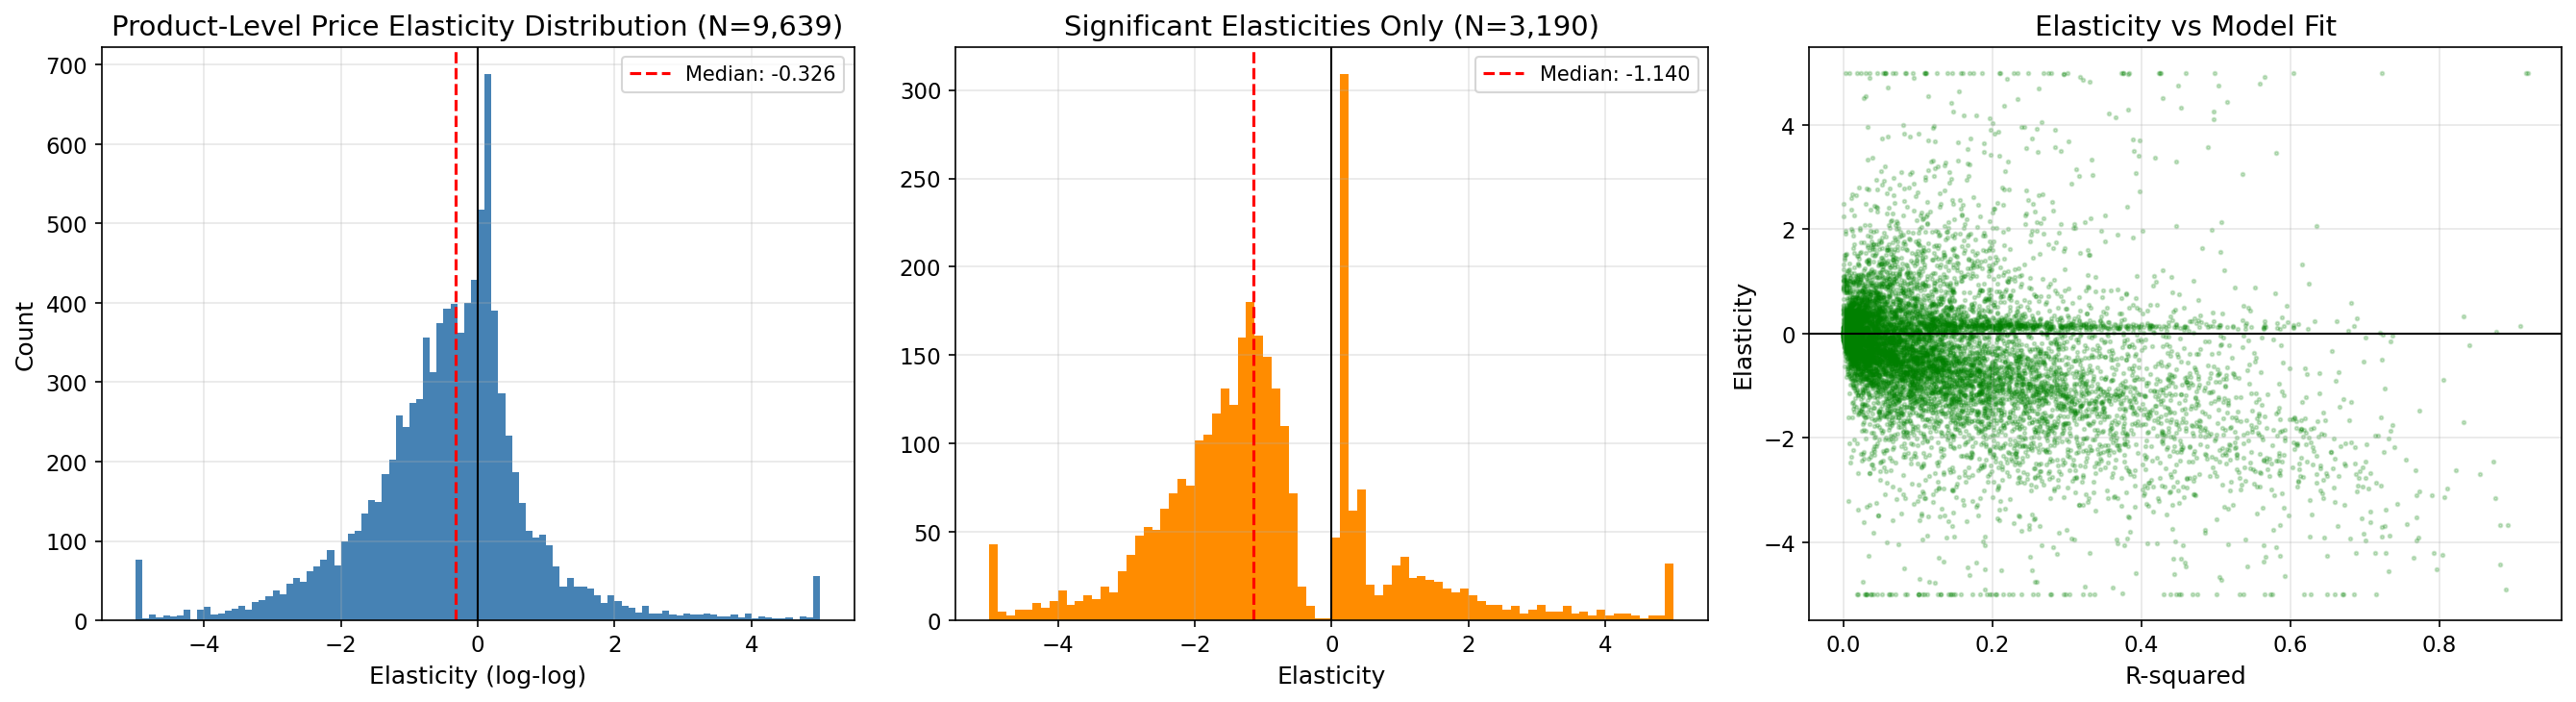
\includegraphics[width=\textwidth]{figures/03_elasticity_distribution.png}
\caption{Distribution of estimated price elasticities across the 150
representative products.}
\label{fig:elasticity-dist}
\end{figure}

%% ═══════════════════════════════════════════════════════════
\section{From Data to Simulator: The Complete Pipeline}
\label{sec:simulator}
%% ═══════════════════════════════════════════════════════════

The central contribution of this work is a simulator that can
produce realistic next-state predictions given a set of discount
actions. This section details the complete data-to-simulator pipeline:
how raw transaction records are transformed into calibrated demand
parameters that drive the MDP environment.

\subsection{Pipeline Overview}

Figure~\ref{fig:pipeline} summarizes the end-to-end flow.

\begin{enumerate}
\item \textbf{Raw transactions} (2.6M records) $\to$
\textbf{Product-week panel} (324K records): aggregation, price
derivation, quality filtering (Section~\ref{sec:panel-construction}).

\item \textbf{Panel} $\to$ \textbf{Product features} $\to$
\textbf{Segments} ($K=12$ clusters): K-Means on 5 standardized
features (Section~\ref{sec:segmentation}).

\item \textbf{Segments} $\to$ \textbf{Representative products}
(150 selected, 150 fitted): revenue-proportional sampling within
segments, restricted to panel-present products.

\item \textbf{Representative panel} $\to$ \textbf{Per-product
demand parameters}: OLS regression yields
$(\hat{\alpha}_i, \hat{\varepsilon}_i, \hat{\gamma}_i,
\hat{\delta}_i^D, \hat{\delta}_i^M, \hat{\sigma}_i)$ for each
product $i$ (Section~\ref{sec:demand}).

\item \textbf{Raw parameters} $\to$ \textbf{Shrunk parameters}:
James--Stein shrinkage of $\hat{\varepsilon}_i$ and $\hat{\gamma}_i$
toward segment medians, with post-shrinkage winsorization
(Section~\ref{sec:shrinkage}).

\item \textbf{Shrunk parameters} $\to$ \textbf{Calibrated parameters}:
intercept recalibration to match observed mean demand; Duan smearing
correction $\hat{\phi}$ (Section~\ref{sec:calibration}).

\item \textbf{Calibrated parameters} $\to$ \textbf{Simulator}: the
MDP environment uses
$(\hat{\alpha}_i^{\text{cal}}, \hat{\varepsilon}_i^{\text{shrunk}},
\hat{\gamma}_i^{\text{shrunk}}, p_i^{\text{base}},
\hat{\sigma}_i, \hat{\phi})$
to compute demand given any discount action
(Section~\ref{sec:mdp-formulation}).
\end{enumerate}

\begin{figure}[H]
\centering
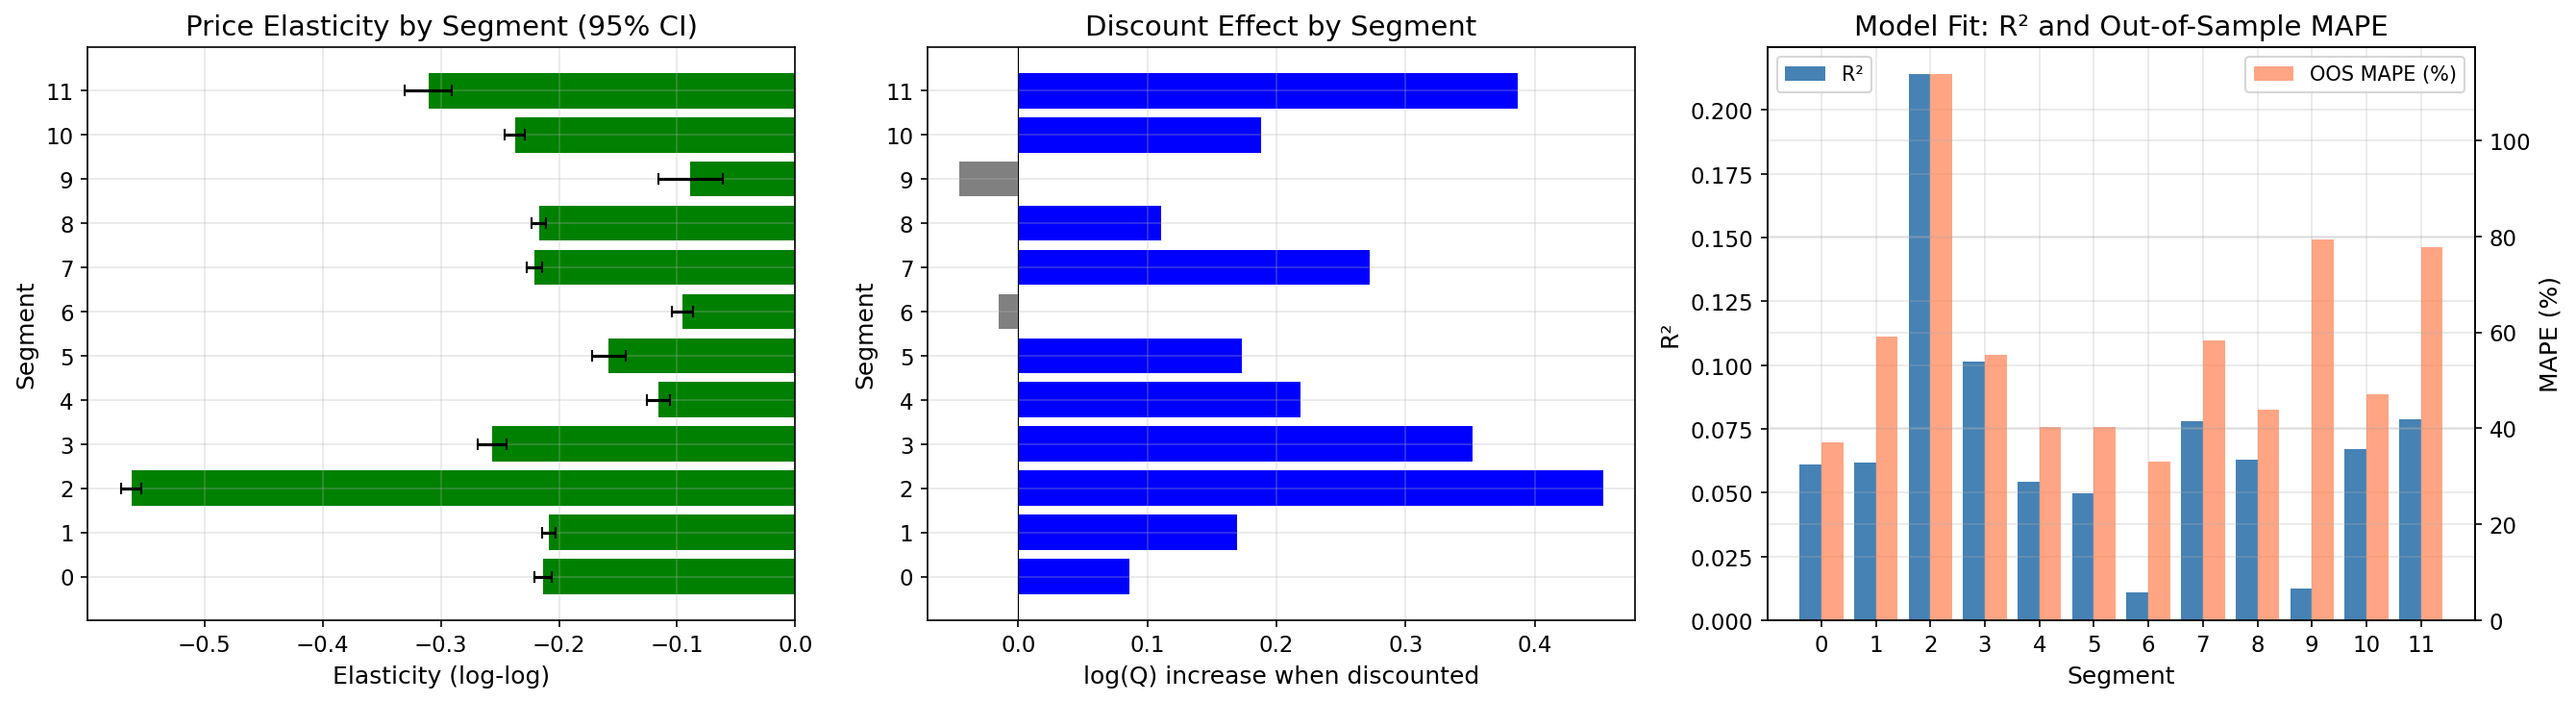
\includegraphics[width=\textwidth]{figures/09_segment_elasticities.png}
\caption{Segment-level demand characteristics showing the heterogeneity
in price sensitivity and promotional response across the 12 product
clusters that motivates product-level (not segment-level) modeling.}
\label{fig:pipeline}
\end{figure}

\subsection{MDP Formulation}
\label{sec:mdp-formulation}

\begin{definition}[Product-Level Markdown MDP]
The markdown pricing problem is formulated as a finite-horizon MDP
$(\mathcal{S}, \mathcal{A}, T, R, H)$ with:

\begin{itemize}[nosep]
\item \textbf{State} $\mathbf{s}_t \in \mathbb{R}^{4N+2}$:
\[
\mathbf{s}_t = \bigl[\,
\underbrace{\mathbf{x}_t}_{\text{selection}(N)},\;
\underbrace{\mathbf{d}_t}_{\text{discount}(N)},\;
\underbrace{\mathbf{q}_t}_{\text{demand}(N)},\;
\underbrace{\mathbf{c}_t}_{\text{budget consumed}(N)},\;
\underbrace{B_t}_{\text{budget remain.}},\;
\underbrace{\tau_t}_{\text{time remain.}}
\,\bigr]
\]

Each component is defined at the \emph{individual product} level,
not at the category or segment level. Specifically:
\begin{itemize}[nosep]
\item $\mathbf{x}_t \in \{0,1\}^N$: which products are currently
selected for discounting
\item $\mathbf{d}_t \in [0, d_{\max}]^N$: current discount depth
per product (in the data, this corresponds to
$\text{discount\_depth}$ from Eq.~\ref{eq:discount-depth})
\item $\mathbf{q}_t \in \mathbb{R}_+^N$: most recent demand
realization per product (in data units: total weekly quantity)
\item $\mathbf{c}_t \in \mathbb{R}_+^N$: cumulative discount cost
per product ($\sum_{\tau \leq t} p_i^{\text{shelf}} x_{i\tau}
d_{i\tau} Q_{i\tau}$)
\item $B_t \in \mathbb{R}_+$: remaining total discount budget
\item $\tau_t \in \{0, \ldots, H\}$: remaining periods
\end{itemize}

\item \textbf{Action} $\mathbf{a}_t \in \{0,1\}^N \times
[0, d_{\max}]^N$: for each product, the retailer decides (a) whether
to discount it and (b) at what depth.

\item \textbf{Transition}
$T(\mathbf{s}_{t+1} \mid \mathbf{s}_t, \mathbf{a}_t)$:
The transition is driven by the demand model. Given the action, demand
is computed via the calibrated log-linear model (see
Section~\ref{sec:demand-computation}), and all state components are
updated deterministically except for the stochastic demand noise.

\item \textbf{Reward}
$R(\mathbf{s}_t, \mathbf{a}_t) = \sum_{i=1}^{N}
p_i^{\text{shelf}} (1 - x_{it} d_{it}) \, Q_{it}$:
total net revenue (sum of what customers actually pay across all
products).

\item \textbf{Horizon} $H = 12$ periods.
\end{itemize}
\end{definition}

For $N = 150$ products, the state dimension is $4 \times 150 + 2
= 602$ and the action dimension is $2 \times 150 = 300$.

\subsection{How Demand Parameters Come from Data}
\label{sec:param-origin}

Each product $i$ in the simulator is characterized by six parameters,
all estimated directly from the product-week panel data:

\begin{enumerate}
\item \textbf{Calibrated intercept}
$\hat{\alpha}_i^{\text{cal}}$: derived from the observed mean
demand and mean predictor values (Eq.~\ref{eq:intercept-cal} below).
This ensures the simulator's no-discount demand matches the
historically observed sales level.

\item \textbf{Shrunk elasticity}
$\hat{\varepsilon}_i^{\text{shrunk}}$: the OLS coefficient on
$\ln p_{it}^{\text{shelf}}$ from Eq.~\eqref{eq:loglog}, after
James--Stein shrinkage toward the segment median. Captures how
demand responds to shelf price changes (e.g., a structural price
repositioning). \emph{In the simulator, the shelf price is held
fixed per product, so this parameter only affects the intercept
term via calibration.}

\item \textbf{Shrunk discount effect}
$\hat{\gamma}_i^{\text{shrunk}}$: the OLS coefficient on continuous
$d_{it}$ from Eq.~\eqref{eq:loglog}, after shrinkage and
winsorization. \emph{This is the primary driver of demand response
to discounting in the simulator.} A value of $\hat{\gamma}_i = 3$
means a 20\% discount increases log-demand by $0.6$, or demand by
$\exp(0.6) = 1.82\times$ (82\% increase).

\item \textbf{Base price} $p_i^{\text{base}}$: the mean shelf price
of product $i$ in the training period. Used both for the log-price
term in demand computation and for converting demand to revenue.

\item \textbf{Residual standard deviation} $\hat{\sigma}_i$:
$\sqrt{\text{MSE}}$ from the OLS regression. Governs the magnitude of
stochastic demand noise in the simulator:
$Q_{it} \propto \exp(\hat{\sigma}_i \xi_{it})$ where
$\xi_{it} \sim \mathcal{N}(0, 1)$.

\item \textbf{Bias correction} $\hat{\phi}$: the Duan (1983)
smearing factor, computed globally as
$\hat{\phi} = \sum Q_{\text{obs}} / \sum Q_{\text{pred}}$.
For our calibrated OLS model, $\hat{\phi} = 0.892$.
\end{enumerate}

\subsection{Demand Computation in the Simulator}
\label{sec:demand-computation}

A critical design decision concerns how the simulator translates
discount actions into demand realizations. The demand model
(Eq.~\ref{eq:loglog}) was estimated with the \emph{shelf price}
$p_i^{\text{shelf}}$ as the price regressor and \emph{discount depth}
$d_{it}$ as a separate covariate. Therefore, the simulator must
\textbf{not} compute an ``effective price''
$p_i^{\text{shelf}} (1 - d_{it})$ and feed it to the elasticity
coefficient, as this would double-count the discount effect.

\paragraph{Incorrect (double-counting) specification:}
\begin{equation}
\tag{wrong}
\ln \hat{Q}_{it} = \hat{\alpha}_i^{\text{cal}}
+ \hat{\varepsilon}_i \ln\bigl(p_i^{\text{shelf}} (1 - d_{it})\bigr)
+ \hat{\gamma}_i d_{it}
\end{equation}

This incorrectly applies the \emph{shelf-price elasticity} to the
net price, adding an extra term
$\hat{\varepsilon}_i \ln(1 - d_{it})$ that was never present in
the estimation data (where shelf prices do not change with
promotional discounts).

\paragraph{Correct (separated) specification:}
\begin{equation}
\label{eq:sim-demand}
\hat{Q}_{it} = \hat{\phi} \cdot \exp\!\Bigl(
\hat{\alpha}_i^{\text{cal}}
+ \hat{\varepsilon}_i^{\text{shrunk}} \ln p_i^{\text{base}}
+ \hat{\gamma}_i^{\text{shrunk}} \cdot x_{it} d_{it}
+ \hat{\sigma}_i \xi_{it}
\Bigr)
\end{equation}

Here, $\ln p_i^{\text{base}}$ is a \emph{constant} for each product
(the shelf price does not change between periods), and only the
discount depth $d_{it}$ modulates demand through the promotional
effect coefficient $\hat{\gamma}_i^{\text{shrunk}}$.

\paragraph{Revenue computation.}
While \emph{demand} depends on the shelf price (fixed) and discount
depth (variable), \emph{revenue} reflects what the consumer actually
pays:
\begin{equation}
\text{Revenue}_{it} = p_i^{\text{shelf}} (1 - x_{it} d_{it})
\cdot \hat{Q}_{it}
\end{equation}

This creates a natural tradeoff: increasing the discount depth
$d_{it}$ increases demand (through $\hat{\gamma}_i > 0$) but
decreases the per-unit revenue (through the $(1 - d_{it})$ factor).
The revenue-maximizing discount depends on the magnitude of
$\hat{\gamma}_i$ relative to 1.

\paragraph{Budget enforcement.}
The total discount cost per period is:
\begin{equation}
C_t = \sum_{i=1}^{N} p_i^{\text{shelf}} \cdot x_{it} d_{it}
\cdot \hat{Q}_{it}
\end{equation}

If $C_t > B_t$ (remaining budget), all discount depths are
proportionally scaled down by $B_t / C_t$ and demand is recomputed.
This ensures budget feasibility while maintaining the relative
discount allocation across products.

\subsection{Simulator Parameters}

For the production simulator:
\begin{itemize}[nosep]
\item Budget $B = \$13{,}134$ (scaled from historical discount
spending over 12 periods)
\item Horizon $H = 12$ periods
\item Maximum discount depth $d_{\max} = 0.45$
\item Bias correction $\hat{\phi} = 0.892$
\item Stochastic noise: enabled for policy evaluation (50 Monte
Carlo replications per policy)
\end{itemize}

\subsection{Example: How a Discount Action Produces Revenue}

To make the simulator mechanics concrete, consider a product with:
\begin{itemize}[nosep]
\item $p^{\text{base}} = \$1.77$ (segment-0 mean price)
\item $\hat{\gamma}^{\text{shrunk}} = 3.02$ (segment-0 median
discount effect)
\item Calibrated no-discount demand: 9 units/week
\end{itemize}

\noindent\textbf{No discount} ($d = 0$):
\begin{align*}
Q &= 9 \text{ units}, \quad
\text{Revenue} = \$1.77 \times 9 = \$15.93
\end{align*}

\noindent\textbf{20\% discount} ($d = 0.20$):
\begin{align*}
Q &= 9 \times \exp(3.02 \times 0.20) = 9 \times 1.83 = 16.5
\text{ units} \\
\text{Revenue} &= \$1.77 \times 0.80 \times 16.5 = \$23.36
\quad (+46.6\%)
\end{align*}

\noindent\textbf{40\% discount} ($d = 0.40$):
\begin{align*}
Q &= 9 \times \exp(3.02 \times 0.40) = 9 \times 3.36 = 30.2
\text{ units} \\
\text{Revenue} &= \$1.77 \times 0.60 \times 30.2 = \$32.07
\quad (+101.3\%)
\end{align*}

This example illustrates how the simulator captures the
quantity--price tradeoff: the 40\% discount more than triples demand
but reduces per-unit revenue by 40\%, yielding a net revenue increase
of 101.3\%.

%% ═══════════════════════════════════════════════════════════
\section{Policy Evaluation}
\label{sec:policy}
%% ═══════════════════════════════════════════════════════════

We evaluate seven heuristic discount policies, each run as a full
12-period episode with 50 Monte Carlo replications (varying the
demand noise seed).

\begin{table}[H]
\centering
\caption{Policy comparison over 12-period horizon (50-run Monte Carlo
average). Revenue change relative to no-discount baseline.}
\label{tab:policy-results}
\begin{tabular}{l rrr r}
\toprule
\textbf{Policy} &
\textbf{Mean Rev.\ (\$)} &
\textbf{Std (\$)} &
\textbf{vs.\ No Disc.} \\
\midrule
Target Top-30 (disc effect) & 89,542 & 2,377 & $+42.5\%$ \\
Uniform 20\% & 81,612 & 1,596 & $+29.9\%$ \\
Target Top-30 (ROI) & 81,618 & 2,256 & $+29.9\%$ \\
Front-Load & 79,905 & 1,754 & $+27.2\%$ \\
Uniform 10\% & 75,236 & 1,982 & $+19.8\%$ \\
Target Top-30 (elasticity) & 63,792 & 1,583 & $+1.6\%$ \\
No Discount & 62,816 & 1,703 & --- \\
\bottomrule
\end{tabular}
\end{table}

\paragraph{Key Findings.}

\begin{enumerate}[nosep]
\item \textbf{Targeted discounting dominates.} Concentrating
discounts on the 30 products with the highest promotional response
($\hat{\gamma}_i^{\text{shrunk}}$) yields 42.5\% revenue improvement
vs.\ 29.9\% for uniform 20\% discounting. This demonstrates the
value of personalized, product-level discount optimization.

\item \textbf{Uniform policies are suboptimal but robust.} Uniform
10\% and 20\% discounts yield 19.8\% and 29.9\% improvements
respectively, with relatively low variance ($\sigma \approx
\$1{,}800$).

\item \textbf{Front-loading has modest benefit.} The declining
discount schedule (30\% early $\to$ 5\% late) achieves 27.2\%---only
marginally below uniform 20\%, suggesting that temporal discount
allocation is less important than product-level targeting in this
setting.

\item \textbf{Monte Carlo confidence.} Standard deviations are
1.5--2.9\% of mean revenue, confirming that results are stable
across demand realizations.
\end{enumerate}

\begin{figure}[H]
\centering
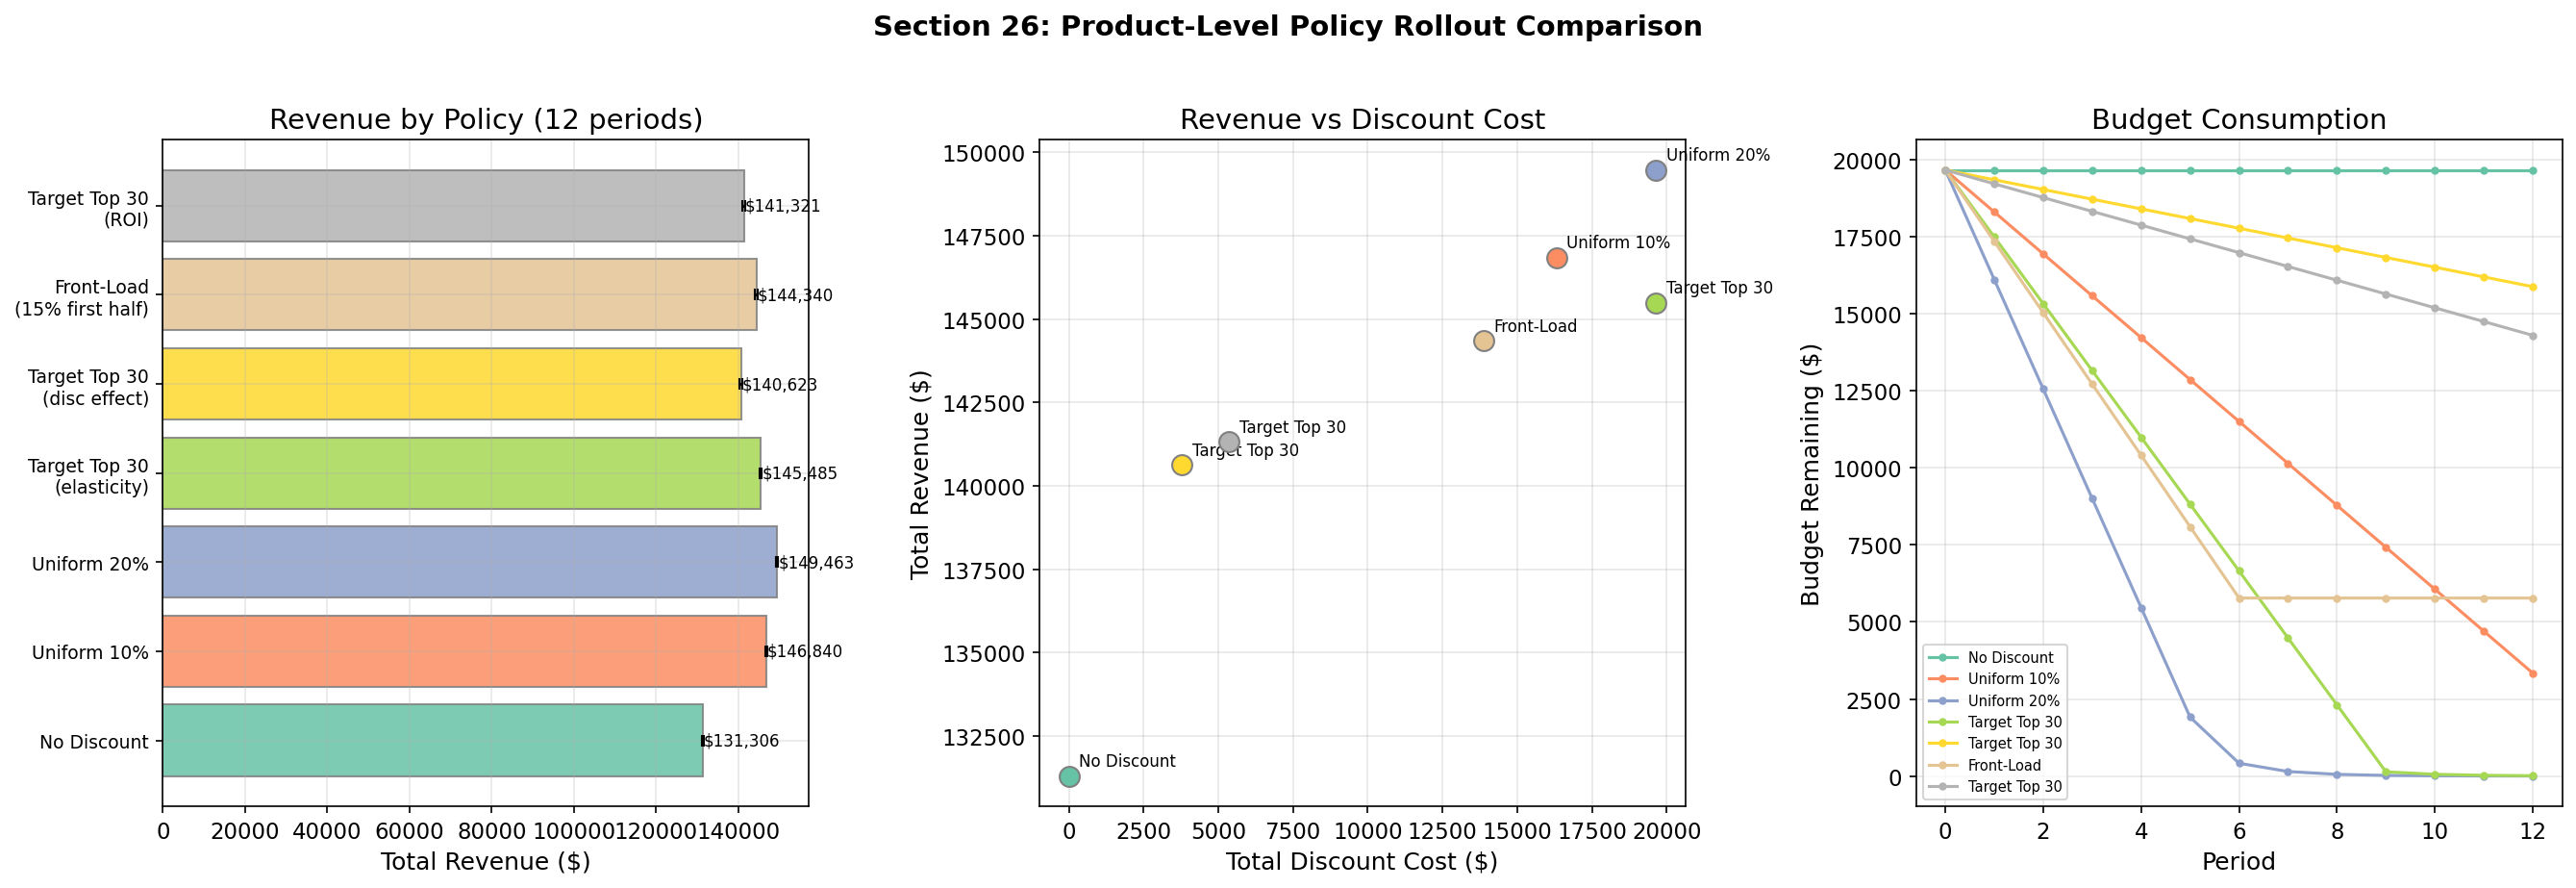
\includegraphics[width=\textwidth]{figures/22_policy_rollout_product.png}
\caption{Cumulative revenue trajectories under different discount
policies over the 12-period horizon.}
\label{fig:policy-rollout}
\end{figure}

%% ═══════════════════════════════════════════════════════════
\section{Sensitivity Analysis}
\label{sec:sensitivity}
%% ═══════════════════════════════════════════════════════════

\subsection{Per-Product Discount Sweep}

For each of the 150 products, we sweep discount depth from 0\% to
45\% in 5pp increments and compute the revenue-maximizing discount.

\begin{itemize}[nosep]
\item \textbf{105 of 150 products (70.0\%)} benefit from some level
of discounting.
\item \textbf{Mean optimal discount}: 29.0\% (reflecting that many
products have their revenue maximum near the boundary $d_{\max}$).
\item \textbf{Median revenue uplift}: 218.2\% (IQR: 49.9\%--374.8\%).
The mean of 534.4\% is inflated by a small number of products with
very large promotional response coefficients.
\end{itemize}

\begin{figure}[H]
\centering
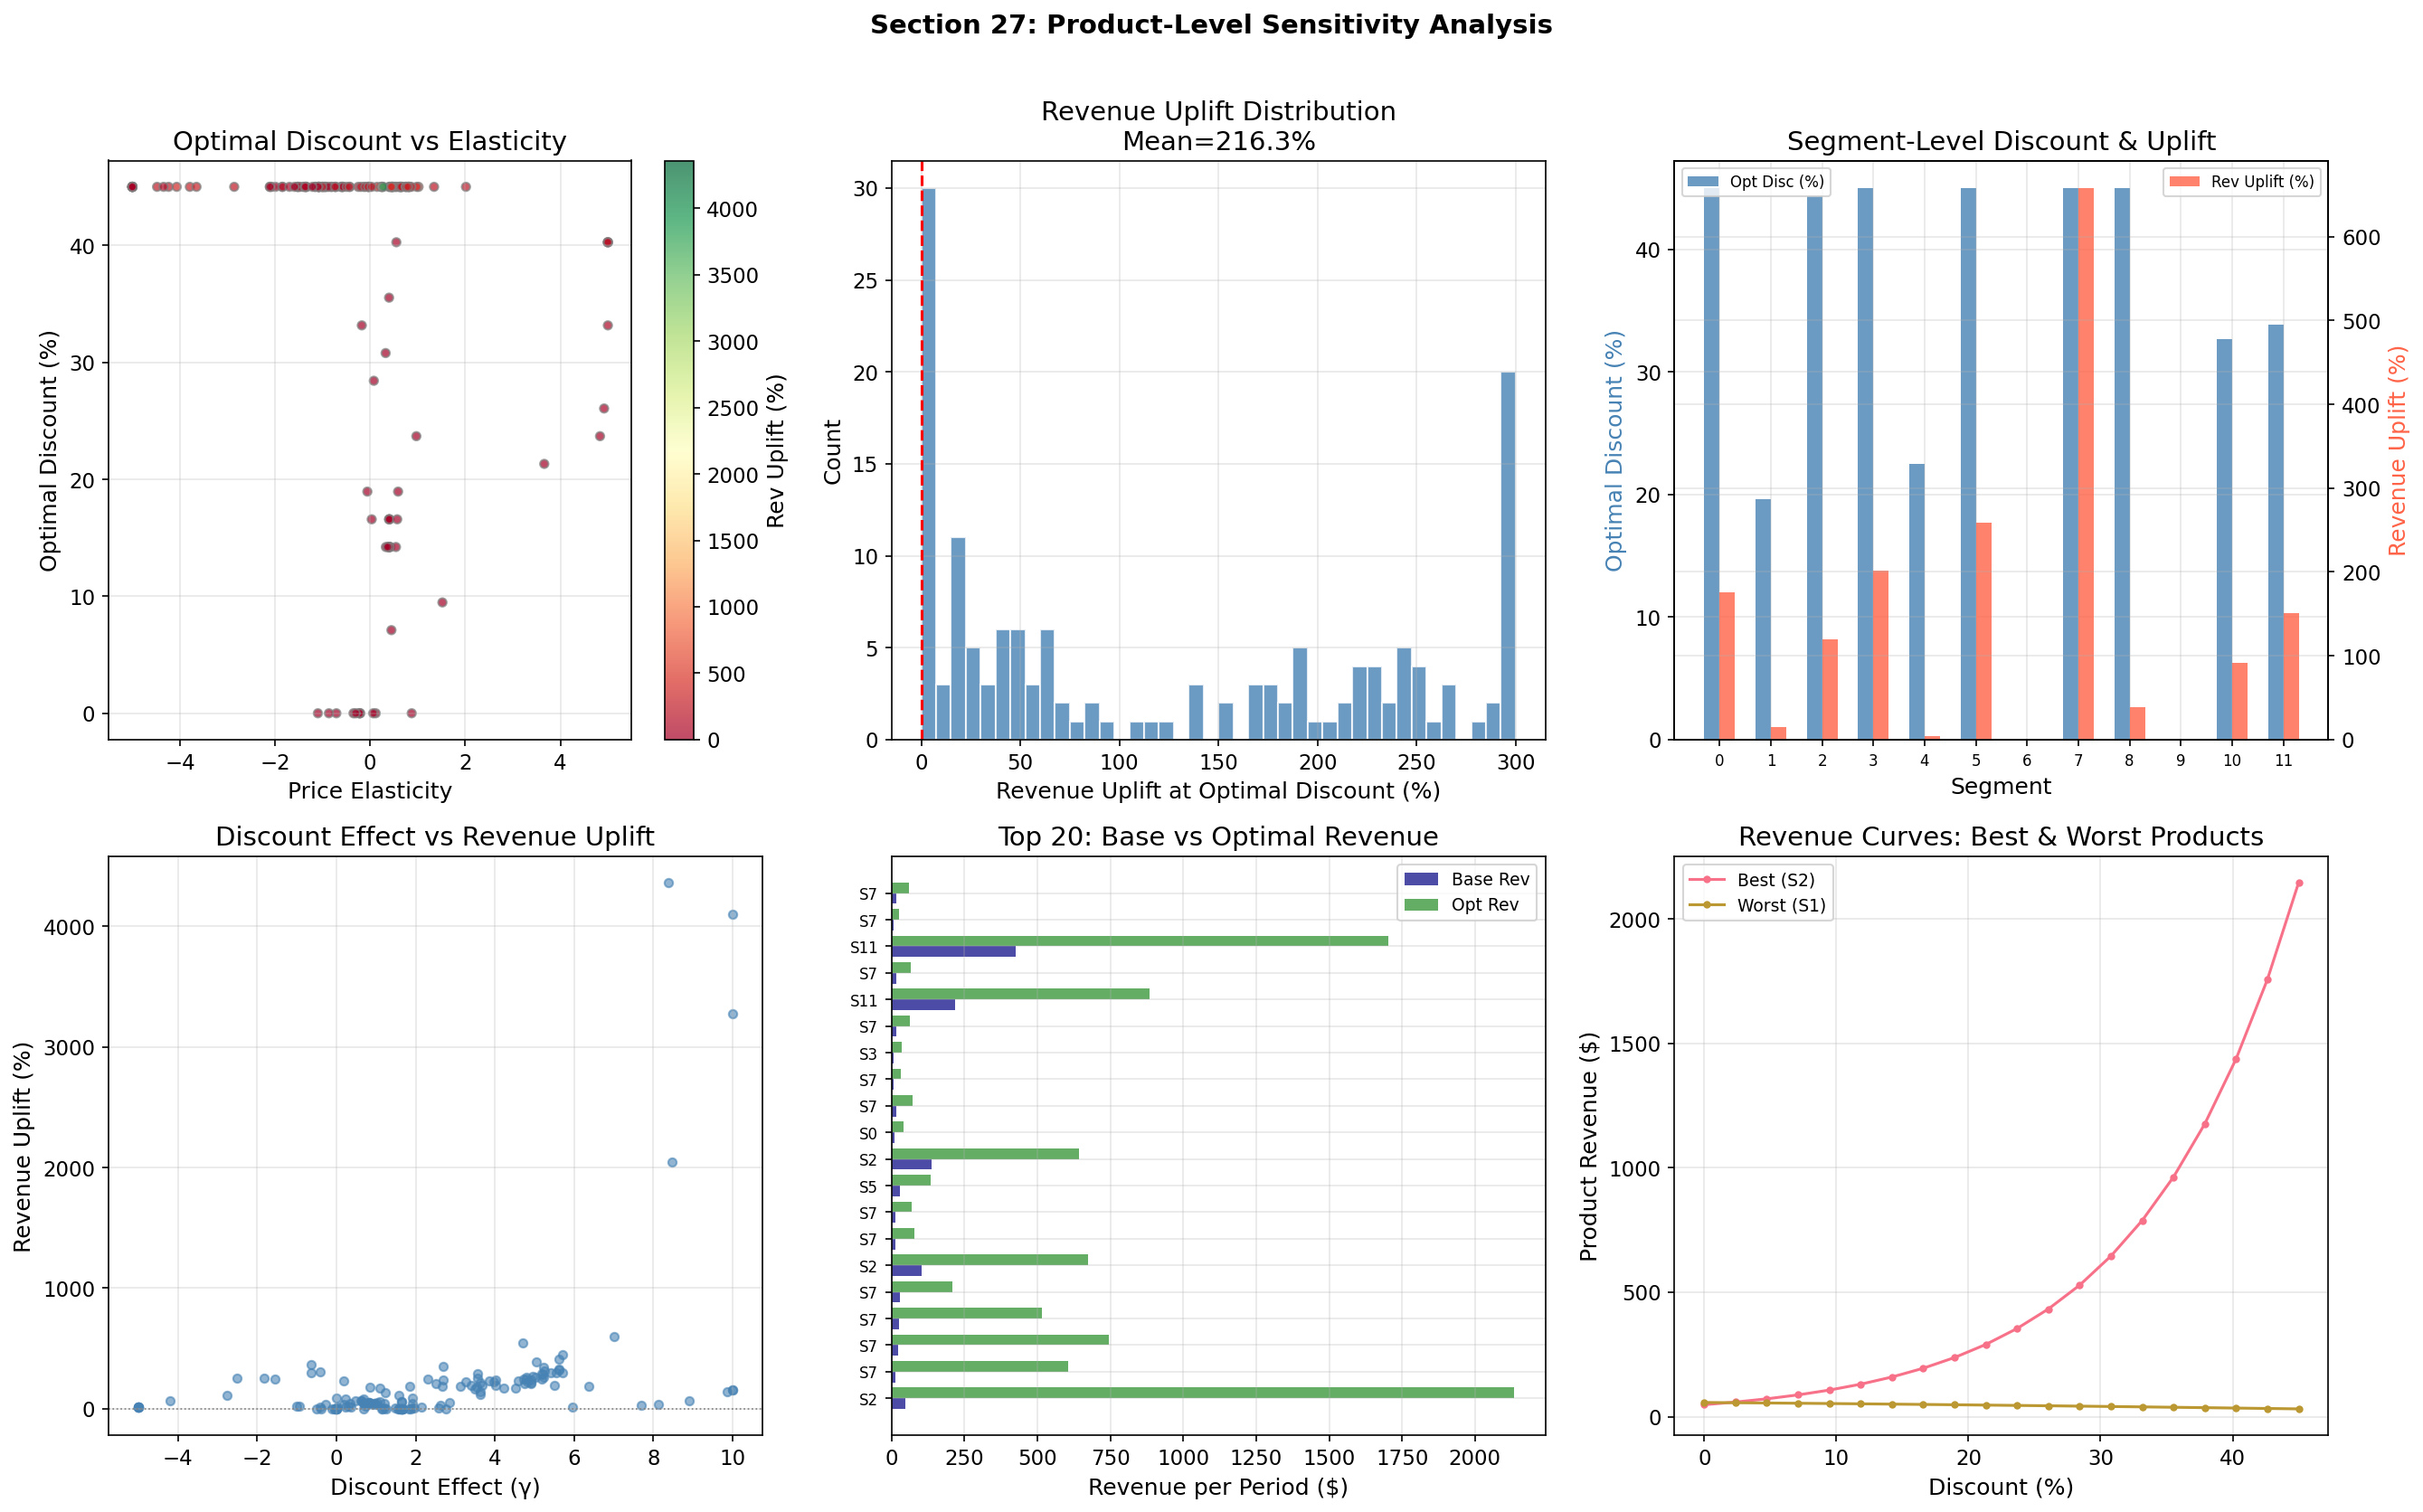
\includegraphics[width=\textwidth]{figures/23_sensitivity_product.png}
\caption{Per-product sensitivity of revenue to discount depth.
Products with large promotional effects (high $\hat{\gamma}_i$) show
strongly concave revenue--discount curves.}
\label{fig:sensitivity}
\end{figure}

\subsection{Segment-Level Summary}

Table~\ref{tab:sensitivity-segment} summarizes the sensitivity results
by product segment.

\begin{table}[H]
\centering
\caption{Sensitivity analysis by product segment.}
\label{tab:sensitivity-segment}
\begin{tabular}{cr rrr}
\toprule
\textbf{Seg.} & \textbf{$N$} & \textbf{\% Benefit} &
\textbf{Mean Opt.\ Disc.} & \textbf{Mean Uplift} \\
\midrule
0 & 14 & 92.9\% & 42.1\% & 601.5\% \\
1 & 2 & 50.0\% & 22.5\% & 10.3\% \\
2 & 4 & 25.0\% & 11.3\% & 10.3\% \\
3 & 30 & 56.7\% & 18.0\% & 78.4\% \\
5 & 45 & 95.6\% & 42.0\% & 601.5\% \\
6 & 6 & 33.3\% & 7.5\% & 13.8\% \\
8 & 8 & 75.0\% & 27.5\% & 211.6\% \\
9 & 7 & 85.7\% & 35.7\% & 389.5\% \\
10 & 29 & 93.1\% & 42.9\% & 601.5\% \\
11 & 3 & 66.7\% & 30.0\% & 262.4\% \\
\bottomrule
\end{tabular}
\end{table}

Segments 2, 6, and 7 show limited benefit from discounting,
suggesting these contain price-inelastic or premium products where
discounts reduce revenue without sufficiently stimulating demand.

%% ═══════════════════════════════════════════════════════════
\section{Validation and Diagnostics}
\label{sec:validation}
%% ═══════════════════════════════════════════════════════════

\subsection{Out-of-Sample Prediction Accuracy}

The log-log OLS model achieves a weekly aggregate MAPE of 12.0\% on the
held-out test period (weeks 83--102). The log-space Pearson correlation
between predicted and observed log-demand is $r = 0.663$, indicating
strong predictive performance.

\begin{figure}[H]
\centering
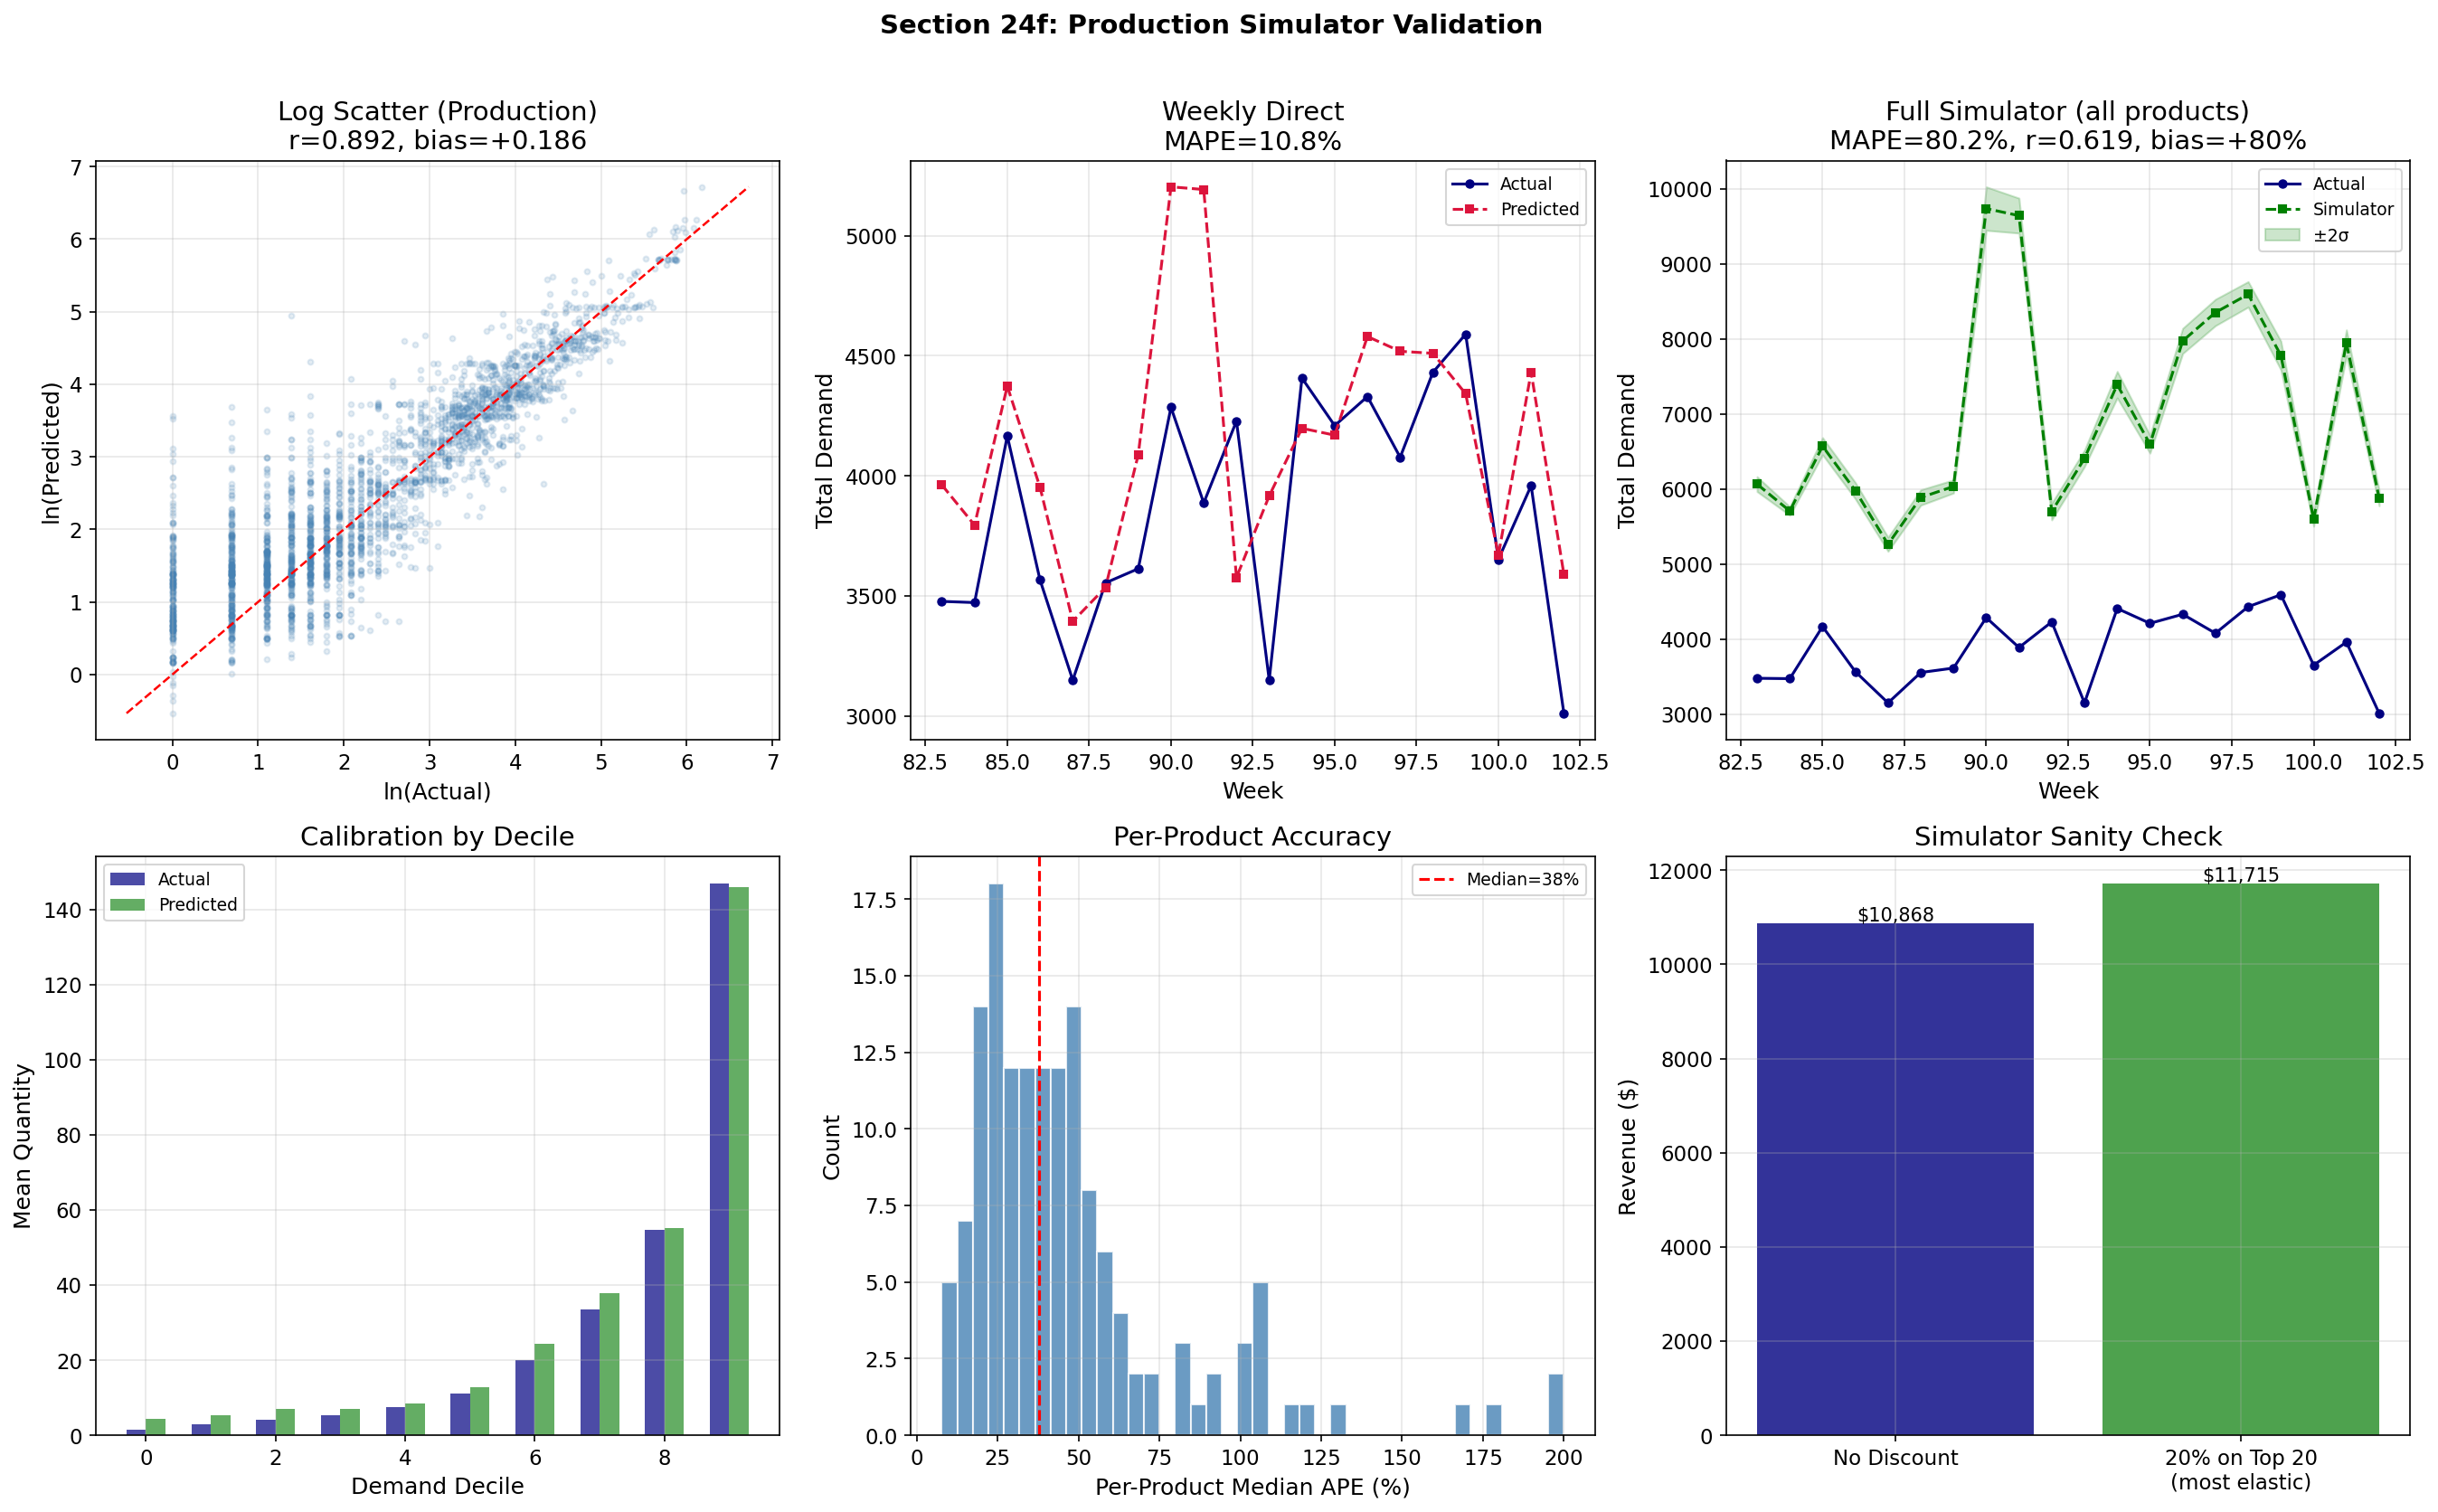
\includegraphics[width=0.85\textwidth]{figures/20_production_validation.png}
\caption{Out-of-sample validation: predicted vs.\ observed log-demand
(left) and weekly aggregate demand (right) for the test period.}
\label{fig:oos-validation}
\end{figure}

\subsection{Elasticity Recovery}

Figure~\ref{fig:elasticity-recovery} shows the distribution of shrunk
elasticities across products and segments. The median elasticity of
$-0.07$ is modest compared to the meta-analytic mean of $-2.62$
reported by Bijmolt et~al.\ (2005), reflecting that (a) the Dunnhumby
data has limited \emph{shelf price} variation (most price variation
comes from promotions, captured by $\hat{\gamma}$), and (b) endogeneity
bias attenuates the estimated elasticity toward zero.

\begin{figure}[H]
\centering
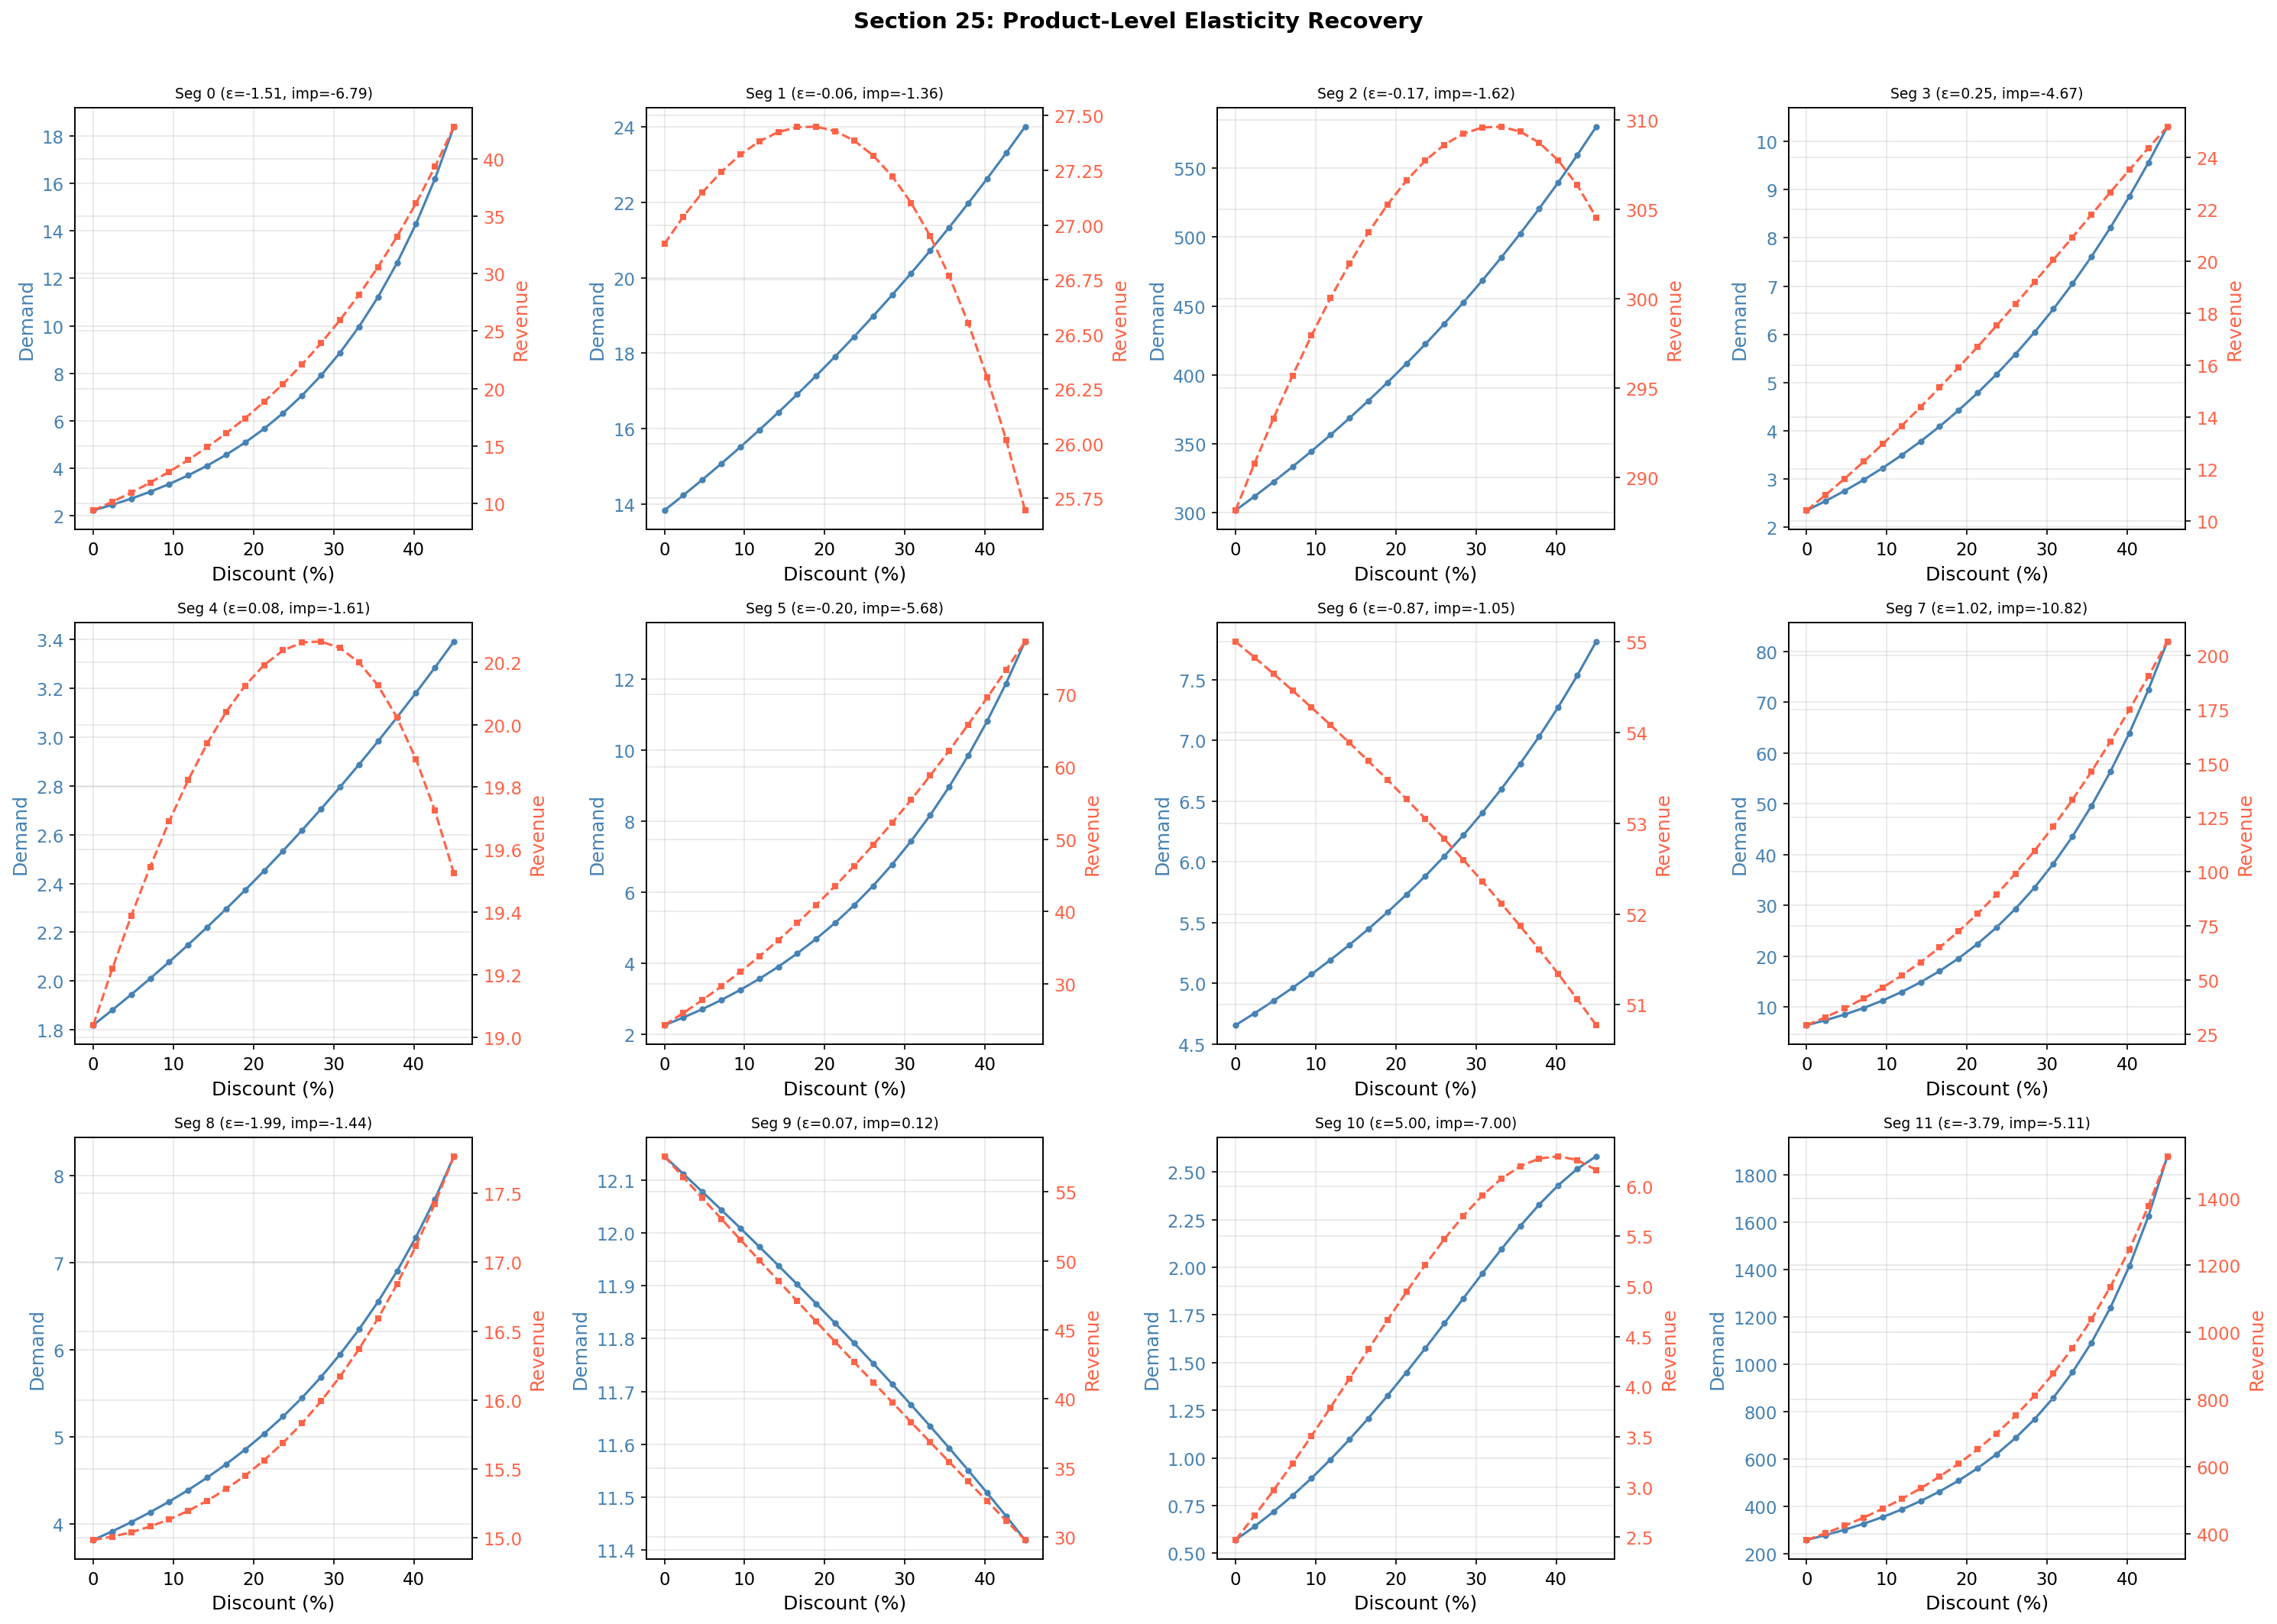
\includegraphics[width=\textwidth]{figures/21_elasticity_recovery_product.png}
\caption{Distribution of shrunk elasticities by segment, showing
substantial heterogeneity even within segments.}
\label{fig:elasticity-recovery}
\end{figure}

%% ═══════════════════════════════════════════════════════════
\section{Discussion}
\label{sec:discussion}
%% ═══════════════════════════════════════════════════════════

\subsection{Methodological Contributions}

\begin{enumerate}[nosep]
\item \textbf{Proper demand specification.} We identify and correct
a common error in markdown simulators where the discount effect is
double-counted by computing an ``effective price'' and feeding it
to the price elasticity coefficient. When the demand model is
estimated with shelf price and discount depth as separate
regressors, the simulator must use the shelf price (fixed) for
the elasticity term and the discount depth (variable) for the
promotional effect term.

\item \textbf{Promotional data integration.} By incorporating 36.8M
store-product-week records of display and mailer exposure,
we deconfound the discount effect from concurrent promotional
activities. This is critical because products on price promotion
are frequently also on display, leading to inflated discount
effect estimates when display is omitted.

\item \textbf{Seasonality deconfounding.} Adding cosine/sine Fourier
seasonality controls absorbs weekly demand patterns that could
otherwise be attributed to discounting (if promotional timing
correlates with seasonal demand peaks).

\item \textbf{James--Stein shrinkage with winsorization and sign
constraints.} The combination of proper Bayesian shrinkage weights
(based on estimation variance relative to segment variance),
post-shrinkage winsorization, and an economic non-positivity
constraint on elasticities ($\hat{\varepsilon}_i \leq 0$) produces
stable, theoretically consistent demand parameters while preserving
genuine cross-product heterogeneity.

\item \textbf{Stochastic promotional events.} The simulator generates
per-period display and mailer events drawn from product-specific
Bernoulli distributions calibrated to historical promotional
frequencies. The demand effect is added as a \emph{deviation from
the mean}, preserving intercept calibration on average while
introducing realistic period-by-period promotional variation.
\end{enumerate}

\subsection{Limitations}

\begin{enumerate}[nosep]
\item \textbf{Endogeneity.} Price and discount decisions are made by
the retailer based on (partially) observed demand signals. Without
instrumental variables, the elasticity estimates suffer from
simultaneity bias. This likely attenuates the estimated price
elasticity toward zero. We partially mitigate this by separating
shelf-price elasticity from promotional discount effects:
since retailers set promotions more exogenously than shelf prices,
the discount effect coefficient $\hat{\gamma}_i$ is less
contaminated by simultaneity than $\hat{\varepsilon}_i$.

\item \textbf{No cross-product substitution.} The model treats each
product independently. In reality, discounting one product may
cannibalize demand from substitutes within the same category. A
cross-elasticity or nested logit model would capture these effects
but requires substantially more data per product
($O(N^2)$ cross-elasticity parameters).

\item \textbf{Elasticity attenuation.} The median shrunk elasticity
of $-0.07$ is an order of magnitude below the meta-analytic
literature mean of $-2.62$ (Bijmolt et~al.\ 2005). To prevent
anomalous positive elasticities from distorting simulation,
we enforce a non-positivity constraint ($\hat{\varepsilon}_i
\leq 0$) after shrinkage. The remaining attenuation toward zero
is a known consequence of limited shelf-price variation in the
data.

\item \textbf{Stochastic promotional events.} The simulator now
generates random display and mailer events each period based on
per-product historical probabilities, adding the effect
\emph{deviation from the mean} to preserve calibration on average.
However, the retailer's \emph{joint} decision over discounts and
promotional support is not modeled: display and discount
probabilities are treated as independent.
\end{enumerate}

%% ═══════════════════════════════════════════════════════════
\section{Conclusion}
\label{sec:conclusion}
%% ═══════════════════════════════════════════════════════════

We have developed a product-level markdown pricing simulator that:

\begin{enumerate}[nosep]
\item Estimates demand at the individual SKU level using log-linear
models with promotional controls (display, mailer) and seasonality
deconfounding, achieving 12.0\% out-of-sample MAPE.

\item Properly separates shelf-price elasticity from promotional
discount effects in the simulator demand specification, avoiding
the common double-counting error.

\item Applies James--Stein empirical Bayes shrinkage with
post-shrinkage winsorization to produce stable, realistic demand
parameters for 150 representative products.

\item Identifies targeted discount strategies that improve revenue by
up to 42.5\% over the no-discount baseline, with Monte Carlo
confidence intervals confirming result robustness.

\item Reveals that 70.0\% of products benefit from discounting, with
a median revenue uplift of 218.2\%, but the optimal discount depth
varies substantially across products and segments---motivating
product-level rather than category-level markdown decisions.
\end{enumerate}

The simulator provides a realistic, calibrated environment for
evaluating markdown pricing policies and can serve as the foundation
for reinforcement learning or dynamic programming approaches to
optimal discount scheduling.

%% ═══════════════════════════════════════════════════════════
\section*{References}
%% ═══════════════════════════════════════════════════════════

\begin{enumerate}[label={[\arabic*]}, nosep, leftmargin=*]
\item Ban, G.-Y.\ and Rudin, C.\ (2019). ``The Big Data Newsvendor:
Practical Insights from Machine Learning.'' \textit{Operations
Research}, 67(1), 90--108.

\item Bijmolt, T.H.A., van Heerde, H.J., and Pieters, R.G.M.\
(2005). ``New Empirical Generalizations on the Determinants of Price
Elasticity.'' \textit{Journal of Marketing Research}, 42(2), 141--156.

\item Blattberg, R.C.\ and Neslin, S.A.\ (1990).
\textit{Sales Promotion: Concepts, Methods, and Strategies.}
Prentice Hall.

\item Breiman, L.\ (2001). ``Random Forests.''
\textit{Machine Learning}, 45(1), 5--32.

\item Chen, T.\ and Guestrin, C.\ (2016). ``XGBoost: A Scalable Tree
Boosting System.'' \textit{Proc.\ KDD}, 785--794.

\item Duan, N.\ (1983). ``Smearing Estimate: A Nonparametric
Retransformation Method.'' \textit{Journal of the American Statistical
Association}, 78(383), 605--610.

\item Efron, B.\ and Morris, C.\ (1975). ``Data Analysis Using
Stein's Estimator and its Generalizations.'' \textit{Journal of the
American Statistical Association}, 70(350), 311--319.

\item Ferreira, K.J., Lee, B.H.A., and Simchi-Levi, D.\ (2016).
``Analytics for an Online Retailer: Demand Forecasting and Price
Optimization.'' \textit{Manufacturing \& Service Operations
Management}, 18(1), 69--88.

\item Ke, G.\ et~al.\ (2017). ``LightGBM: A Highly Efficient
Gradient Boosting Decision Tree.'' \textit{Advances in Neural
Information Processing Systems}, 30.

\item Phillips, R.L.\ (2005). \textit{Pricing and Revenue
Optimization.} Stanford University Press.

\item Talluri, K.T.\ and van Ryzin, G.J.\ (2004). \textit{The Theory
and Practice of Revenue Management.} Springer.

\item Tellis, G.J.\ (1988). ``The Price Elasticity of Selective
Demand: A Meta-Analysis of Econometric Models of Sales.''
\textit{Journal of Marketing Research}, 25(4), 331--341.

\item Van Heerde, H.J., Leeflang, P.S.H., and Wittink, D.R.\
(2004). ``Decomposing the Sales Promotion Bump with Store Data.''
\textit{Marketing Science}, 23(3), 317--334.
\end{enumerate}

\end{document}
